% \iffalse meta-comment
%
% Copyright (C) 2026 by ShixuanCheng
%
% This work may be distributed and/or modified under the
% conditions of the LaTeX Project Public License, either version 1.3c
% of this license or (at your option) any later version.
%
% \fi
%
% \iffalse
%<*driver>
\ProvidesFile{hauthesis.dtx}[2026/10/01 v1.0 Huai'an University Thesis Template]
\documentclass{ltxdoc}
\usepackage{dtx-style}

\EnableCrossrefs
\CodelineIndex

\begin{document}
	\DocInput{\jobname.dtx}
\end{document}
%</driver>
% \fi
% 
% \def\indexname{索引}
% \IndexPrologue{\section{\indexname}}
%
% \title{\bfseries\color{haucolor}\hauthesis：淮安大学学位论文模板}
% \author{程世轩\\[5pt] \githubuser{shxuanc}\\[5pt] {3058778192@qq.com}}
% \date{v1.0（2026.10.1）国庆特别版}
% \maketitle
% 
% \vspace{2\baselineskip}
% \begin{center}
%   {\Large\bfseries 摘\quad 要}
% \end{center}
% \vspace{\baselineskip}
% 
% \hauthesis{} 是一个面向淮安大学本科毕业设计（论文）的 \LaTeX{} 模板。
% 它依据学校提供的 Word 模板，逐项测量并复现了页面设置、字号字体、行距、
% 标题层级、页眉页脚、图表与公式编号、参考文献著录等格式要求，
% 并提供了封面、中英文摘要、目录、注释、致谢等部分的现成环境，
% 使用者只需在示例文档中填写内容，无需自行调整版式。
% 
% 本文档是该模板的使用说明与实现记录。
% 前半部分介绍安装与编译方法，后半部分逐节说明各项格式的实现细节，
% 并给出与学校规范中数值的对照，便于使用者核验与自行调整。
% 
% \vspace{2\baselineskip}
% \begin{center}
%   {\Large\bfseries 免责声明}
% \end{center}
% \vspace{\baselineskip}
% 
% \begin{enumerate}
%   \item 本模板的发布遵守 \href{https://www.latex-project.org/lppl/lppl-1-3c.txt}{\LaTeX{} Project Public License (1.3.c)}
%         以及其后的最新版本，使用前请认真阅读协议内容。
% 
%   \item 本模板为作者根据淮安大学教务处颁发的毕业设计（论文）撰写规范
%         与学校提供的 Word 模板编写而成，
%         旨在供淮安大学毕业生撰写毕业设计（论文）使用。
% 
%   \item 淮安大学教务处只提供毕业设计（论文）写作规范与 Word 模板，
%         不提供官方 \LaTeX{} 模板，也不会授权第三方模板为官方模板，
%         所以此模板仅为写作规范的参考实现，不保证格式审查老师不提意见。
%         任何由于使用本模板而引起的论文格式审查问题均与本模板作者无关。
% 
%   \item 任何个人或组织以本模板为基础进行修改、扩展而生成的新专用模板，
%         请严格遵守 \href{https://www.latex-project.org/lppl/lppl-1-3c.txt}{\LaTeX{} Project Public License (1.3.c)}
%         协议以及其后的最新版本。
%         由于违犯协议而引起的任何纠纷争端均与本模板作者无关。
% \end{enumerate}
% 
% \clearpage
% \pagestyle{fancy}
% \begin{multicols}{2}[]
%   \tableofcontents
% \end{multicols}
% \clearpage
%
% \section{模板介绍}
% \hauthesis{}（\textbf{H}uai'\textbf{a}n \textbf{U}niversity \LaTeX{}
% \textbf{Thesis} Template）是为了帮助淮安大学毕业生撰写毕业论文而编写
% 的 \LaTeX{} 论文模板。
% 
% 本模板依据淮安大学教务处发布的本科毕业设计（论文）撰写规范及其配套的
% Word 模板编写，各项版式参数（页边距、字号、行距、标题层级、图表题注、
% 参考文献著录格式等）均按该规范设定。规范若有修订，请以教务处发布的为准，并据此调整模板中的对应参数。
% 
% 模板覆盖论文的全部组成部分：封面、中英文摘要、目录、正文各章、图表与
% 公式、参考文献、注释、总结与展望、致谢以及附录。章节标题、页码编排、
% 页眉页脚、图表编号与交叉引用均由模板自动处理，作者只需专注于内容本身，
% 不必关心版式细节。
% 
% 使用本模板需要 \XeLaTeX{} 编译，参考文献由 biber 处理，
% 建议使用 \TeX{} Live 2023 或更高版本。模板提供了构建脚本，按生成文档类、
% 编译正文、处理文献、再次编译的顺序自动执行。
% 
% \section{贡献者}
% \label{sec:contributors}
%
% \hauthesis{} 的开发过程中，主要的维护者包括：
%
% \begin{itemize}
%   \item 程世轩（\githubuser{shxuanc}）：最早的开发者，2026 年创建 \hauthesis{} 并长期进行维护工作。
% \end{itemize}
% 
% \entry{招募维护者}
% 此外，本模板长期欢迎新的维护者加入。模板涉及版式参数、宏包兼容以及各版本
% \TeX{} Live 的差异，维护工作繁杂，仅靠个人难以覆盖所有使用场景与反馈。
% 
% 有意参与者最好具备以下基础：一是能够读懂 \LaTeX{} 宏包与文档类的源码，
% 看得懂 \file{.dtx} 与 \file{.cls} 文件的组织方式；二是了解 \pkg{ctex} 宏集的
% 标题、字号与页面机制，因为本模板由 \pkg{ctexbook} 派生而来；三是会使用
% Git 进行版本管理并提交修改；四是愿意耐心核对版式细节，并记录每处改动的
% 依据。其中前两项可以在参与过程中逐步熟悉，并不构成入门门槛。
% 
% 联系方式：GitHub \githubuser{shxuanc}，邮箱 \href{mailto:3058778192@qq.com}{3058778192@qq.com}。
%
% \section{安装}
% \label{sec:installation}
%
% \StopEventually{\PrintIndex}
% 
% \subsection{环境要求}
% \label{sec:requirements}
% 
% 建议使用 \TeX{} Live 发行版，2023 年或更高版本。其他发行版一般也可以使用，
% 但未经充分测试。编译引擎使用 \XeLaTeX{}，参考文献默认使用 biber 处理，
% 两者在 \TeX{} Live 中随发行版一同安装，无需另外配置。
% 
% 模板通过 \pkg{ctex} 宏集排版中文，在 Windows、macOS 与 Linux 上均可使用，但是还是建议使用 Windows 系统进行写作。
% 
% \subsection{获取模板}
% \label{sec:get-template}
% 
% 从项目仓库下载源码包并解压，解压后的主要文件与目录见下表：
% 
% \begin{longtable}{ll}
%   \toprule
%   文件或目录 & 用途 \\
%   \midrule
%   \endfirsthead
%   \multicolumn{2}{r}{\footnotesize 续表} \\
%   \toprule
%   文件或目录 & 用途 \\
%   \midrule
%   \endhead
%   \midrule
%   \multicolumn{2}{r}{\footnotesize 续下页} \\
%   \endfoot
%   \bottomrule
%   \endlastfoot
%   \file{.vscode/}				& VSCode 配置文件 \\
%   \file{code/}						& 代码文件 \\
%   \file{contents/}			& 各章节的内容文件，一章一个文件。 \\
%   \file{figures/}				& 插图文件。 \\
%   \file{reference/}			& 参考文献数据文件（\file{.bib}）。 \\
%   \file{main.tex}				& 论文的主文件，作者在此组织全文结构。 \\
%   \file{main.pdf}				& 示例论文，由\file{main.tex}编译产出。 \\
%   \file{hauthesis.cls}	& 论文类文件，主文档基于改类文件写作。 \\
%   \file{latexmkrc}			& \pkg{latexmk} 的配置文件。 \\
%   \file{Makefile}				& 构建脚本，Windows 需要安装 GNU make 工具 \\
%   \file{make.bat}				& Windows 下的构建脚本。 \\
%   \file{hauthesis.pdf}	& 说明文档，由\file{hauthesis.dtx}编译产出。 \\
%   \file{hauthesis.dtx}	& 模板的全部源码与说明文档，是唯一的源文件。 \\
%   \file{hauthesis.ins}	& 用于从 \file{.dtx} 中提取 \file{.cls} 的脚本。 \\
%   \file{README.md}			& 项目说明。 \\
% \end{longtable}
% 
% \subsection{生成文档类}
% \label{sec:generate-cls}
% 
% \file{hauthesis.dtx} 是文档化源码，不能直接供 \cs{documentclass } 调用，
% 需先用 \texttt{DocStrip} 拆包，生成 \file{hauthesis.cls}：
% 
% \begin{shell}
%   latex hauthesis.ins
% \end{shell}
% 
% \subsection{编译论文}
% \label{sec:generate-thesis}
% 
% 只需在 \file{main.tex} 中组织章节顺序，具体内容写在 \file{contents/}
% 目录下各自的文件里，然后进行编译，\hauthesis 提供了多种编译方式。
% 
% \subsubsection{latexmk}
% \label{sec:latexmk}
% 
% \entry{latexmk}
% \hauthesis{} 提供了 \file{latexmkrc} 文件，\pkg{latexmk} 会自动判断需要编译几次、何时调用 biber，
% 一条命令即可完成全部步骤：
% \begin{shell}
%   latexmk main.tex				# 生成示例论文 main.pdf
%   latexmk thuthesis.dtx		# 生成说明文档 hauthesis.pdf
%   latexmk -c							# 清理编译生成的辅助文件
% \end{shell}
% 常用参数如下：
% 
% \begin{description}
%   \item[\texttt{-xelatex}] 指定使用 \XeLaTeX{} 引擎编译。
%   \item[\texttt{-pvc}] 持续监听源文件，改动后自动重新编译。
%   \item[\texttt{-c}] 删除编译产生的辅助文件，保留 \file{.pdf}。
%   \item[\texttt{-C}] 连同 \file{.pdf} 一并删除，即彻底清理。
% \end{description}
% 
% \subsubsection{GNU make}
% \label{sec:make}
% 
% \entry{GNU mak}
% 若在 Windows 下安装了 GNU Make，则可与 Linux、macOS 一样，直接使用模板提供的 \file{Makefile}：
% 
% \begin{shell}
%   make all					# doc + thesis（等价于 make doc thesis）
%   make cls					# latex hauthesis.ins —— 生成 .cls 与 dtx-style.sty
%   make doc					# 先生成类，再编译两遍 hauthesis.dtx → hauthesis.pdf
%   make thesis				# 先生成类，再 xelatex → biber → xelatex ×2 → main.pdf
%   make clean				# 清理辅助文件
% \end{shell}
% 参数如下：
% \begin{description}
%   \item[\texttt{thesis}] 编译论文。
%   \item[\texttt{cls}] 只生成文档类 \file{hauthesis.cls}。
%   \item[\texttt{doc}] 生成说明文档 \file{hauthesis.pdf}。
%   \item[\texttt{all}] 依次完成上述全部工作。
%   \item[\texttt{clean}] 删除辅助文件，保留 \file{.pdf}。
%   \item[\texttt{help}] 显示各目标的说明。
% \end{description}
% 
% \subsubsection{make.bat}
% \label{sec:make-bat}
% 
% \entry{make.bat}
% \hauthesis{} 为 Windows 用户提供了 \file{make.bat}，对上述编译链进行了封装。
% 在 PowerShell 或者 cmd 中调用：
% 
% \begin{shell}
%   .\make.bat cls				# latex hauthesis.ins —— 生成 .cls 与 dtx-style.sty
%   .\make.bat doc				# 先生成类，再编译两遍 hauthesis.dtx → hauthesis.pdf
%   .\make.bat thesis			# 先生成类，再 xelatex → biber → xelatex ×2 → main.pdf
%   .\make.bat all				# doc + thesis（等价于 make doc thesis）
%   .\make.bat clean			# 清理辅助文件
% \end{shell}
% 
% 直接输入 \texttt{make.bat} 在 \env{powershell} 中会提示找不到命令，
% 因为 Windows 默认不把当前目录列入可执行文件的搜索路径。
% 写成 \texttt{./make.bat} 虽然多数情况下也能执行，
% 但正斜杠并非 Windows 的路径分隔符，属于兼容行为。
% 
% \file{make.bat} 的目标与 \file{Makefile} 一致，均为 \texttt{thesis}、
% \texttt{cls}、\texttt{doc}、\texttt{all}、\texttt{clean}。
% 其中 \texttt{clean} 用于删除辅助文件，保留 \file{.pdf}。
% 
% \subsubsection{\XeLaTeX{}}
% \label{sec:manual-chain}
% 
% \entry{\XeLaTeX{}}
% 不使用任何脚本时，需要按以下顺序手动执行，缺一不可：
% 
% \begin{shell}
%   xelatex hauthesis.ins		# 生成 hauthesis.cls
%   xelatex main.tex				# 生成引用与目录数据
%   biber main							# 处理参考文献数据
%   xelatex main.tex				# 排入文献表与交叉引用
%   xelatex main.tex				# 排定页码与书签
% \end{shell}
% 
% 两次 \XeLaTeX{} 不能省略。第一次负责写入交叉引用与目录数据，第二次才把它们
% 排进页面；只编译一次时，正文中的引用编号与目录页码会显示为上一次的结果或问号。
% 
% \subsubsection{VSCode \texttt{settings.json}}
% \label{sec:vscode}
% 
% \entry{\file{settings.json}}
% 若使用 Visual Studio Code 写作，安装 \pkg{LaTeX Workshop} 扩展之后，
% 还需要一份配置告诉它用什么命令、按什么顺序编译。项目自带的
% \file{.vscode/settings.json} 已经写好，打开项目即可使用，不必手动配置。
% 
% \noindent\file{latex-workshop.latex.tools} 一节列出九条命令：
% 
% \begin{description}
%   \item[\texttt{xelatex}] 用 \XeLaTeX{} 编译当前文件。
%   \item[\texttt{hauthesis-ins}] 运行 \file{hauthesis.ins} 解包。
%   \item[\texttt{hauthesis-dtx}] 编译 \file{hauthesis.dtx} 生成手册。
%   \item[\texttt{biber}] 处理参考文献数据。
%   \item[\texttt{bibtex}] 备选，供使用 BibTeX 的情形。
%   \item[\texttt{makeindex}] 生成手册的命令索引。
%   \item[\texttt{latexmk}] 自动判断编译次数。
%   \item[\texttt{pdflatex}、\texttt{lualatex}] 备选引擎。
% \end{description}
% 
% \subsection{生成说明文档}
% \label{sec:generate-doc}
% 
% 说明文档随模板一起下发，若需自行编译本说明文档，执行 \texttt{make.bat doc} 即可。脚本会先生成文档类，
% 再用 \XeLaTeX{} 编译 \file{hauthesis.dtx} 并生成命令索引，得到
% \file{hauthesis.pdf}。
% 
% \section{使用说明}
% \label{sec:usage}
% 
% 本手册假定用户已经能处理一般的 \LaTeX{} 文档，并对 BibTeX 有一定了解。如果
% 从未接触过 \TeX{} 和 \LaTeX，建议先学习相关的基础知识。
% 
% \subsection{文档类选项}
% \label{sec:options}
% 
% \DescribeEnv{documentclass}
% 文档类选项写在 \cs{documentclass} 的方括号内，多个选项之间用逗号分隔：
% \begin{latex}
%   \documentclass[windows]{hauthesis}
% \end{latex}
% 其中 [windows] 为不同操作系统选择，见\ref{sec:os}。
% 
% \subsubsection{操作系统}
% \label{sec:os}
% 
% \entry{操作系统}
% 不同操作系统自带的中英文字体并不相同，因此提供以下四个选项：
% \DescribeMacro{windows}
% \DescribeMacro{macos}
% \DescribeMacro{linux}
% \DescribeMacro{none}
% \begin{description}
%   \item[\option{windows}] \textbf{默认值}，使用 Windows 自带的中文字体（SimSun、SimHei、
%     KaiTi、FangSong 等）。
%   \item[\option{macos}] 使用 macOS 自带的中文字体（Songti SC、Heiti SC、
%     Kaiti SC 等）。
%   \item[\option{linux}] 使用 Fandol 系列字体，随 \TeX{} Live 提供，不必另外安装。
%   \item[\option{none}] 不做任何字体设置，由使用者自行配置。
% \end{description}
% 
% 在 macOS 或 Linux 上写作时，建议显式写出对应选项，避免因缺少 Windows 字体
% 而回退到默认字形，导致版面与预期不符。
% 
% \subsubsection{编号方式}
% \label{sec:numbering}
% 
% \entry{编号方式}
% \DescribeMacro{plainfig}
% \DescribeMacro{plaintab}
% \DescribeMacro{plaineqn}
% \DescribeMacro{plainalg}
% 图、表、公式、算法四者的编号默认都带章号，形如「图 2-1」「式 (2-3)」。
% 若需要改为全文连续编号（「图 1」「式 1」），使用下面四个选项，
% 它们互相独立，可以任意组合：
% 
% \begin{center}
% \begin{tabular}{ll}
%   \toprule
%   选项 & 作用 \\
%   \midrule
%   \option{plainfig} & 图不带章号 \\
%   \option{plaintab} & 表不带章号 \\
%   \option{plaineqn} & 公式不带章号 \\
%   \option{plainalg} & 算法不带章号 \\
%   \bottomrule
% \end{tabular}
% \end{center}
% 
% 例如只让图连续编号，其余三者保持带章：
% 
% \begin{latex}
%   \documentclass[plainfig]{hauthesis}
% \end{latex}
% 
% 四者全部连续编号：
% 
% \begin{latex}
%   \documentclass[plainfig, plaintab, plaineqn, plainalg]{hauthesis}
% \end{latex}
% 
% \textbf{切换编号方式后需要重新编译两遍}，才能让正文中的交叉引用更新。
% 正文里的引用请一律用 \cs{ref}，不要手写「图 2-1」这样的编号，
% 否则切换后文字会对不上。
% 
% \subsubsection{其他选项}
% \label{sec:other-options}
% 
% \entry{ctex}
% 未被模板占用的选项会原样传给 \cls{ctexbook} 文档类，因此 \pkg{ctex} 宏集支持的
% 选项都可以直接使用，例如用 \option{zihao=-4} 指定正文字号、用
% \option{scheme=chinese} 指定章节标题方案。具体取值参见 \pkg{ctex} 宏集的文档。
% 
% \subsection{论文结构}
% \label{sec:structure}
% \entry{main.tex}
% 论文主文件 \file{main.tex} 按前置、主体、后置三部分组织，顺序不能调换：
% 
% \begin{latex}
%  % !TeX encoding = UTF-8
%  % !TeX program  = xelatex
%  
%  \documentclass{hauthesis}
%  
%  \usepackage[backend=biber, style=gb7714-2015]{biblatex}
%  \addbibresource{reference/reference.bib}
%  
%  % 封面字段（正式写论文时替换成自己的信息）
%  \def\YourName{张三}
%  \def\YourNumber{112300000000}
%  \def\YourCollege{电子信息工程学院}
%  \def\YourMajor{人工智能}
%  \def\PaperTitleLa{基于多传感器融合的移动机器人}
%  \def\PaperTitleLb{路径规划与避障算法研究}
%  \def\SupervisorNameIn{某某某}
%  \def\SupervisorTitleIn{教授}
%  \def\SupervisorNameOut{/}
%  \def\SupervisorTitleOut{/}
%  \def\PaperYear{2027}
%  \def\PaperMonth{5}
%  \def\PaperTitleENa{Path Planning and Obstacle Avoidance
%  for Mobile Robots}
%  \def\PaperTitleENb{Based on Multi-Sensor Fusion}
%  \def\Keywords{关键词，关键词，关键词，关键词}
%  \def\KeywordsEN{keyword,\ keyword,\ keyword,\ keyword}
%  
%  \begin{document}
%  
%  \frontmatter % 前置部分（封面、摘要、目录等）
%  
%	 \MakeCover
%	 
%	 \begin{cnabstract}
摘要应能独立成篇，让读者不必通读全文，也能掌握论文的核心信息。
其内容应覆盖与论文相当的主要信息，便于读者判断是否值得进一步阅读，
也便于二次文献引用。摘要通常要写明研究目的、方法、结果和结论，
其中结果和结论是重点。

\textcolor{red}{
说明：要求200$\sim$300字，“关键词”为小四号黑体，关键词的个数为3$\sim$8个。
关键词的排序，通常应按研究的对象、性质（问题）和采取的手段排序，而不应任意排列。
“关键词”后面不加冒号，空连个字符，关键词与关键词之间用全角逗号（，）隔开，
最后一个关键词后不加任何标点。
}

\end{cnabstract}

\begin{enabstract}
This is the English abstract of the thesis. It should summarise the research
problem, the method and the main conclusions of the paper.
\par
New paragraph of the English abstract.

\vspace{2em}
说明：\par 
Keywords 为小四号 Times New Roman，加粗。外文关键词（keyword）一律小写，
并与中文关键词一一对应。\textbf{Keywords} 后面不加冒号，空两个字符，
keyword 与 keyword 之间用半角逗号（,）隔开，每个（,）后空 1 个字符，
最后一个 keyword 后不加任何标点符号。
\par
\textcolor{red}{注意：此处行距已经设置为英文段落的间距
（即基础行距 1.2，行距设置为 1.5 倍行距）。}
\end{enabstract}

%	 
%	 \hautocstart
%	 \tableofcontents
%	 \hautocend
%	 
%	 \mainmatter % 主体部分（章节内容）
%	 
%	 \chapter{绪论}
绪论（引言）部分应如下几个部分：
\begin{enumerate}
  \item 研究背景：即“这个课题为什么重要？”以及研究领域的历史回顾\notemark{1}；
  \item 文献综述：前人工作的综合述评\notemark{2}；
  \item 研究目的：需要解决什么；
  \item 流程方法：说清楚论文所采用的解决方法流程；
  \item 论文结构：整篇论文的组织架构。
\end{enumerate}

\section{研究背景与意义}

随着智能制造与智慧物流的快速发展，移动机器人已广泛应用于仓储搬运、自动配送、巡检
安防等场景\cite{tan2013robot}。路径规划与避障是其实现自主导航的核心环节，直接决定
机器人能否在狭窄通道、密集人流等复杂条件下安全高效地完成任务。然而，依赖单一传感器
的方案普遍存在局限：激光雷达测距精度高，但在长廊等几何特征退化的环境中容易匹配
失败\cite{zhang2014loam,shan2018lego}；视觉相机成本低、信息丰富，却受光照变化与
纹理缺失影响明显\cite{qin2018vins}；惯性测量单元与轮式里程计输出频率高，但存在
累积漂移\cite{fox2005probabilistic}。因此，本文面向低成本移动平台，研究多传感器
融合的定位方法与分层路径规划算法，以提高机器人在动态环境中的定位精度与避障可靠性。

\section{国内外研究现状}

\subsection{多传感器融合定位研究现状}

早期工作多采用扩展卡尔曼滤波融合惯性测量单元与轮式里程计，随后激光雷达被引入，
形成了以扫描匹配为核心的定位与建图方案\cite{zhang2014loam,shan2018lego}。视觉方面，
多状态约束卡尔曼滤波把视觉观测与惯性状态联合优化\cite{mourikis2007msckf}，
VINS-Mono 进一步实现了单目视觉惯性系统的紧耦合估计\cite{qin2018vins}。国内学者在
机器人感知与导航方面也开展了系统研究\cite{tan2013robot,wang2004parallel}。

\subsection{路径规划与避障研究现状}

路径规划可分为全局规划与局部避障两个层次。全局规划的代表性工作是 A* 算法，它通过
启发式函数引导搜索并保证最优性\cite{hart1968formal}；采样类方法如快速扩展随机树
更适合高维与复杂约束问题\cite{lavalle1998rrt}。局部避障方面，动态窗口法在速度空间
中采样并评价候选轨迹，计算量小、响应快\cite{fox1997dw}。

近年来，深度学习方法被广泛引入感知与决策环节\cite{lecun2015deep,he2016deep}，
深度强化学习则被用于序列决策问题\cite{mnih2015human,silver2016go}，其在未知环境中的
路径规划上表现出一定优势；相关理论基础可参见周志华的专著\cite{zhou2016ml}。

\subsection{存在的问题}

综合国内外研究现状可以看出，现有工作仍存在以下缺口。其一，多数融合方案依赖高精度
传感器与精细标定，在低成本平台上的适用性有待验证；其二，全局规划与局部避障往往
分别设计，缺乏统一的分层框架，难以兼顾路径质量与实时性；其三，动态障碍的运动规律
多被简化处理，与真实场景存在差距。本文即针对上述缺口展开研究。

\section{论文主要研究内容}
本文的主要研究内容包括：
\begin{enumerate}
  \item 构建基于多传感器融合的环境感知模型；
  \item 设计面向动态环境的路径规划与避障算法；
  \item 搭建仿真平台验证所提方法的有效性；
  \item 分析不同场景下的规划效果与鲁棒性。
\end{enumerate}

\section{论文组织结构}
本文共分为六章，各章节内容安排略。
%	 \chapter{相关理论基础}

本章介绍后续章节所依赖的理论基础，包括深度学习的基本原理、卷积神经网络、
循环神经网络与强化学习，并结合图示、表格与公式给出必要的数学表述。

\section{深度学习基本原理}

\subsection{神经网络基本结构}

神经网络由若干层神经元堆叠而成。单个神经元先对输入做加权求和，再经激活函数得到输出
\begin{equation}
  y = \sigma\left(\sum_{i=1}^{n} w_i x_i + b\right)
  \label{eq:neuron}
\end{equation}
其中 $w_i$ 为权重，$b$ 为偏置，$\sigma(\cdot)$ 为激活函数。

多层网络把前一层的输出作为后一层的输入，逐层计算得到最终结果。设第 $l$ 层的权重矩阵为
$W^{(l)}$、偏置向量为 $b^{(l)}$，则该层的激活值为
\begin{equation}
  a^{(l)} = \sigma\left(W^{(l)} a^{(l-1)} + b^{(l)}\right)
  \label{eq:forward}
\end{equation}
整个网络的结构如图~\ref{fig:mlp} 所示。

\begin{figure}[htbp]
  \centering
  \includegraphics[width=0.55\linewidth]{duck}
  \caption{前馈神经网络结构示意图}
  \label{fig:mlp}
\end{figure}

\subsection{反向传播算法}

反向传播用于计算损失函数对各层参数的梯度。定义第 $l$ 层的误差项为损失对该层加权输入的偏导
\begin{equation}
  \delta^{(l)} = \frac{\partial C}{\partial z^{(l)}}
  \label{eq:delta}
\end{equation}

误差项由输出层向前逐层递推，相邻两层之间满足
\begin{equation}
  \delta^{(l)} = \left( \left( W^{(l+1)} \right)^{\top} \delta^{(l+1)} \right) \odot \sigma'\left( z^{(l)} \right)
  \label{eq:bp}
\end{equation}
其中 $\odot$ 表示逐元素相乘。

得到误差项后，参数的梯度可按链式法则写出，并沿梯度反方向更新
\begin{equation}
  W^{(l)} \leftarrow W^{(l)} - \eta \, \delta^{(l)} \left( a^{(l-1)} \right)^{\top}
  \label{eq:update}
\end{equation}
其中 $\eta$ 为学习率。学习率过大会引起震荡，过小则收敛缓慢。

\subsection{常用激活函数}

激活函数为网络引入非线性。常用的三种激活函数及其表达式如表~\ref{tab:activation} 所示。

\begin{table}[htbp]
  \centering
  \caption{常用激活函数及其特点}
  \label{tab:activation}
  \begin{tabular}{lll}
    \toprule
    名称 & 表达式 & 特点 \\
    \midrule
    Sigmoid & $\sigma(x) = \dfrac{1}{1 + e^{-x}}$ & 输出范围 $(0,1)$，易饱和 \\
    Tanh & $\tanh(x) = \dfrac{e^{x} - e^{-x}}{e^{x} + e^{-x}}$ & 输出零均值，仍会饱和 \\
    ReLU & $\mathrm{ReLU}(x) = \max(0, x)$ & 计算简单，缓解梯度消失 \\
    \bottomrule
  \end{tabular}
\end{table}

其中 ReLU 因计算代价低且能有效缓解深层网络的梯度消失问题，在卷积网络中应用最为广泛，
其函数图像如图~\ref{fig:relu} 所示，对应的导数为
\begin{equation}
  \mathrm{ReLU}'(x) =
  \begin{cases}
    1, & x > 0 \\
    0, & x \le 0
  \end{cases}
  \label{eq:relu}
\end{equation}

由式~\ref{eq:relu} 可见，正半轴导数恒为 1，梯度可无衰减回传，这正是 ReLU 缓解
梯度消失的原因；而负半轴导数为 0，会使该区域的神经元不再更新。

\begin{figure}[htbp]
  \centering
  \begin{tikzpicture}[scale=1.5, font=\fontsize{10.5pt}{12.6pt}\selectfont]
    \draw[-latex] (-1.3,0) -- (1.9,0) node[right] {$x$};
    \draw[-latex] (0,-0.3) -- (0,1.5) node[left] {$y$};
    \draw[very thick, red] (-1.3,0) -- (0,0) -- (1.4,1.4);
  \end{tikzpicture}
  \caption{ReLU 激活函数图像}
  \label{fig:relu}
\end{figure}

\section{卷积神经网络}

\subsection{卷积操作}

卷积神经网络通过局部连接与权重共享提取空间特征。二维卷积操作可以表示为
\begin{equation}
  (f * g)(i, j) = \sum_{m} \sum_{n} f(m, n) \cdot g(i - m, j - n)
  \label{eq:conv2d}
\end{equation}

在 CNN 中，卷积层的输出为
\begin{equation}
  y_{ij} = \sigma\left( \sum_{m} \sum_{n} w_{mn} \cdot x_{(i+m)(j+n)} + b \right)
  \label{eq:convout}
\end{equation}
卷积核在输入特征图上滑动，同一组权重在整个特征图上重复使用，因此参数量远小于全连接层。

\subsection{池化操作}

池化操作用于降低特征图的空间维度，减少计算量并增强平移不变性。常用的池化方式包括
最大池化与平均池化，分别取窗口内的最大值与平均值
\begin{equation}
  y_{ij} = \max_{(m,n) \in R_{ij}} x_{mn}, \qquad
  y_{ij} = \frac{1}{|R_{ij}|} \sum_{(m,n) \in R_{ij}} x_{mn}
  \label{eq:pool}
\end{equation}
其中 $R_{ij}$ 为第 $(i,j)$ 个池化窗口覆盖的区域，$|R_{ij}|$ 为该区域内的元素个数。
两种池化的效果对比如图~\ref{fig:pool} 所示。

\begin{figure}[htbp]
  \centering
  \begin{subfigure}[b]{0.45\linewidth}
    \centering
    \includegraphics[width=\linewidth,page=1]{abc}
    \caption{最大池化}
    \label{fig:pool-max}
  \end{subfigure}
  \hfill
  \begin{subfigure}[b]{0.45\linewidth}
    \centering
    \includegraphics[width=\linewidth,page=2]{abc}
    \caption{平均池化}
    \label{fig:pool-avg}
  \end{subfigure}
  \caption{两种池化方式的对比}
  \label{fig:pool}
\end{figure}

\subsection{典型网络结构}

随着网络加深，研究者提出了多种改进结构以缓解退化与梯度消失问题。几种典型结构的
特点如表~\ref{tab:cnn} 所示。

\begin{table}[htbp]
  \centering
  \caption{几种典型卷积网络结构的对比}
  \label{tab:cnn}
  \begin{tabular}{cccc}
    \toprule
    网络    & 层数 & 核心思想                        & 提出年份 \\
    \midrule
    AlexNet & 8    & 使用 ReLU 与 Dropout            & 2012     \\
    VGG     & 19   & 用小卷积核堆叠替代大卷积核        & 2014     \\
    ResNet  & 152  & 引入残差连接，缓解深层退化        & 2015     \\
    \bottomrule
  \end{tabular}
\end{table}

\section{循环神经网络}

\subsection{RNN 基本结构}

循环神经网络（Recurrent Neural Network, RNN）是处理序列数据的重要模型。RNN 通过
引入循环连接，使网络具有记忆功能。其隐藏状态按时刻递推，输出由当前隐藏状态决定
\begin{equation}
  h_t = \tanh\left( W_h h_{t-1} + W_x x_t + b \right), \qquad y_t = W_y h_t + b_y
  \label{eq:rnn}
\end{equation}
其中 $x_t$ 为 $t$ 时刻的输入，$h_{t-1}$ 为上一时刻的隐藏状态。
若进一步考虑输出层，则 RNN 的完整前向传播可写为
\begin{equation}
  \begin{aligned}
    h_t &= \tanh(W_h h_{t-1} + W_x x_t + b_h), \\
    \hat{y}_t &= \mathrm{softmax}(W_o h_t + b_o).
  \end{aligned}
\end{equation}

\subsection{LSTM 与 GRU}

标准 RNN 在序列较长时容易出现梯度消失或爆炸。长短期记忆网络通过输入门、遗忘门与
输出门控制信息的流动
\begin{equation}
  \begin{aligned}
    f_t &= \sigma\left( W_f \left[ h_{t-1}, x_t \right] + b_f \right) \\
    i_t &= \sigma\left( W_i \left[ h_{t-1}, x_t \right] + b_i \right) \\
    o_t &= \sigma\left( W_o \left[ h_{t-1}, x_t \right] + b_o \right)
  \end{aligned}
  \label{eq:lstm}
\end{equation}

门控循环单元则把三个门简化为更新门与重置门两个，在保持性能的同时减少了参数量。
三种结构的对比如表~\ref{tab:rnn} 所示。

\begin{table}[htbp]
  \centering
  \caption{RNN、LSTM 与 GRU 的结构对比}
  \label{tab:rnn}
  \begin{tabular}{lccc}
    \toprule
    结构 & 门控数量 & 参数量 & 长序列表现 \\
    \midrule
    RNN  & 0 & 最少 & 较差 \\
    LSTM & 3 & 最多 & 好   \\
    GRU  & 2 & 中等 & 好   \\
    \bottomrule
  \end{tabular}
\end{table}

\section{强化学习基本原理}

\subsection{马尔可夫决策过程}

强化学习通常建模为马尔可夫决策过程，由状态集、动作集、转移概率与奖励函数构成。
在策略 $\pi$ 下，状态价值函数定义为折扣回报的期望
\begin{equation}
  V^{\pi}(s) = \mathbb{E}_{\pi}\left[ \sum_{k=0}^{\infty} \gamma^{k} r_{t+k} \,\middle|\, s_t = s \right]
  \label{eq:value}
\end{equation}
其中 $\gamma \in [0,1)$ 为折扣因子，用于权衡当前奖励与未来奖励。

价值函数满足贝尔曼方程，把当前时刻的期望回报拆成即时奖励与下一时刻价值之和
\begin{equation}
  V^{\pi}(s) = \sum_{a} \pi(a \mid s) \sum_{s'} p(s' \mid s, a) \left[ r(s,a,s') + \gamma V^{\pi}(s') \right]
  \label{eq:bellman}
\end{equation}

\subsection{Q 学习算法}

Q 学习直接估计动作价值函数 $Q(s,a)$，不需要知道环境模型。它按时序差分误差更新，
用下一时刻的最大动作价值作为当前估计的目标
\begin{equation}
  Q(s_t, a_t) \leftarrow Q(s_t, a_t) + \alpha \left[ r_t + \gamma \max_{a'} Q(s_{t+1}, a') - Q(s_t, a_t) \right]
  \label{eq:qlearning}
\end{equation}
其中 $\alpha$ 为学习率。当动作空间或状态空间连续时，可以用函数逼近代替查表。

\subsection{深度 Q 网络}

深度 Q 网络用神经网络参数化动作价值函数 $Q(s,a;\theta)$，通过最小化时序差分误差训练
\begin{equation}
  L(\theta) = \mathbb{E}\left[ \left( r_t + \gamma \max_{a'} Q(s_{t+1}, a'; \theta^{-}) - Q(s_t, a_t; \theta) \right)^{2} \right]
  \label{eq:dqn}
\end{equation}
其中 $\theta^{-}$ 为目标网络的参数，定期从当前网络复制，以减小训练过程中的震荡。

\section{本章小结}

本章介绍了深度学习与强化学习的基本原理，给出了神经元模型、前向传播、反向传播、
卷积与池化、循环网络以及价值函数与 Q 学习的数学表述，并通过图示与表格对比了
典型网络结构的特点，为后续章节的算法设计提供理论依据。

%	 \chapter{补充说明}

\section{梯度下降}

梯度下降是一种一阶迭代优化方法：每步沿损失函数梯度的反方向调整参数，使损失
逐步下降。算法~\ref{alg:gd} 给出其基本流程，每轮迭代先计算当前参数处的梯度，
再按学习率 $\eta$ 成比例地更新参数，梯度项的逐分量推导见附录~\ref{app:gd}。

学习率决定每步的跨度：取值过大时损失可能震荡甚至发散，过小时收敛缓慢。
实践中通常在梯度项上引入动量，或改用自适应学习率的方法，以兼顾收敛速度
与稳定性。

\begin{algorithm}[htbp]
  \caption{梯度下降}
  \label{alg:gd}
  \begin{algorithmic}[1]
    \Require 训练集 $D = \{(x^{(i)}, y^{(i)})\}_{i=1}^{m}$，
             学习率 $\eta$，迭代次数 $T$
    \Ensure 参数 $\theta$
    \State 随机初始化 $\theta$
    \For{$t = 1$ \textbf{to} $T$}
      \State 计算梯度
             $\nabla J(\theta) = \frac{1}{m}\sum_{i=1}^{m}
              \left( h(x^{(i)}) - y^{(i)} \right) x^{(i)}$
      \State 更新参数 $\theta \gets \theta - \eta \nabla J(\theta)$
      \If{$\lVert \nabla J(\theta) \rVert < \varepsilon$}
        \State \textbf{break}
      \EndIf
    \EndFor
    \State \Return $\theta$
  \end{algorithmic}
\end{algorithm}

%	 
%	 \begin{conclusion}

本文围绕移动机器人在复杂环境下的自主导航问题，完成了理论梳理、多传感器融合定位与
路径规划避障三部分工作。理论方面汇总了神经网络、卷积与循环网络以及强化学习的数学
表述；定位方面建立了多传感器的时间同步与外参标定流程，采用误差状态卡尔曼滤波融合
激光雷达、惯性测量单元与轮式里程计，实验表明定位误差较单一传感器降低三成以上；
规划方面在 A$^{*}$ 算法的代价函数中引入转向惩罚项，并在动态窗口法中加入全局路径
引导项，仿真显示狭窄通道下的通行成功率明显提高。相对于任务书的要求，本文的实验
均在室内结构化环境完成，未引入视觉信息，动态障碍的运动规律也与真实行人存在差距。
后续可引入视觉惯性里程计、把方法扩展到多机器人协同，并研究外参在线标定与参数选取
的理论依据。

\textcolor{red}{说明：总结与展望，总结课题完成了哪些相关工作，得到的成果如何（或得到了什么结论），相对于任务书要求，还存在哪些不足；可以提出建议、研究设想、改进思路、尚待解决的问题等等。}

\end{conclusion}

%	 \begin{acknowledgements}

四年的本科学习即将结束，毕业论文的完成也得到了许多人的帮助，在此谨致谢意。

首先感谢我的指导教师某某某教授。从选题的确定、方案的论证到论文的反复修改，
老师都给予了耐心细致的指导。老师严谨的治学态度与务实的工作作风，使我在专业
知识之外受益更多。

感谢实验室的各位同学，在程序调试与实验数据整理过程中给予的帮助；也感谢同宿舍
的朋友们，四年朝夕相处，彼此扶持。

感谢我的父母。他们在我求学期间始终给予理解与支持，使我能够安心完成学业。

最后，感谢所有在论文写作过程中提供帮助的老师与同学。

\end{acknowledgements}

%	 \begin{notes}

\item 背景要引用权威的文献和数据，不要写“人工智能很重要”这类空话。

\item 需要指出存在的缺口，指向研究目的。

\end{notes}

%	 
%	 \printbibliography
%	 
%	 \appendix

\chapter{补充推导}

\section{梯度下降的推导}
\label{app:gd}

对均方误差损失
\begin{equation}
  J(\theta) = \frac{1}{2m}\sum_{i=1}^{m}\left(h(x^{(i)}) - y^{(i)}\right)^2
  \label{eq:appendix-mse}
\end{equation}
求关于第 $j$ 个参数的偏导，可得
\begin{equation}
  \frac{\partial J(\theta)}{\partial \theta_j}
  = \frac{1}{m} \sum_{i=1}^{m}
    \left( h(x^{(i)}) - y^{(i)} \right) x_j^{(i)}
  \label{eq:appendix-grad}
\end{equation}
式~\ref{eq:appendix-grad} 即梯度项的逐分量形式。

\section{反向传播的链式法则}

略。

\subsection{三级子标题（条目）}

略

\chapter{补充数据}

\section{实验参数}

模型训练使用的主要参数见表~\ref{tab:appendix-params}。

\begin{table}[htbp]
  \centering
  \caption{训练参数设置}
  \label{tab:appendix-params}
  \begin{tabular}{ccc}
    \hline
    编号 & 参数 & 数值 \\
    \hline
    1 & 学习率   & 0.01 \\
    2 & 批大小   & 64   \\
    3 & 迭代次数 & 1000 \\
    \hline
  \end{tabular}
\end{table}

\section{补充结果}

\begin{figure}[htbp]
  \centering
  \includegraphics[width=0.225\linewidth,page=3]{abc}
  \caption{附图}
  \label{fig:futu}
\end{figure}

\chapter{代码示例}

\section{代码块}

\begin{lstlisting}[language=Python]
for (int i = 0; i < n; i++) {
  sum += a[i] * w[i];   # 累加加权和
}
\end{lstlisting}

\begin{lstlisting}[language=Python,numbers=none]
for (int i = 0; i < n; i++) {
  sum += a[i] * w[i];   # 累加加权和
}
\end{lstlisting}

\section{等宽字体及代码配色}

\begin{lstlisting}[language=Python, style=codeMono]
for (int i = 0; i < n; i++) {
  sum += a[i] * w[i];   # 累加加权和
}
\end{lstlisting}

\hautocodestyle[vscode]

\begin{lstlisting}[language=JavaScript, style=codeMono]
const sig = x => 1 / (1 + Math.exp(-x));            // sigmoid 激活函数
const pred = (X, w) => X.map(r => sig(r.reduce((s, v, i) => s + v * w[i], 0)));
const loss = (X, y, w) => -y.reduce((s, v, i) => s + v * Math.log(pred(X, w)[i]), 0) / y.length;
const X = [[1,0],[0,1],[1,1]], y = [1,0,1];
let w = [0,0];
for (let t = 0; t < 100; t++) {
  w = w.map((v, j) => v - 0.1 * X.reduce((s, r, i) => s + (pred(X, w)[i] - y[i]) * r[j], 0) / y.length);
}
console.log("权重:", w);                             // 输出结果
console.log("损失:", loss(X, y, w));
\end{lstlisting}

\section{引入代码文件}

\hautocodestyle[print]

\codeinputhl[language=python, numbers=none]{code/test.py}

\hautocodestyle[classic]

\codeinputhl[language=python, style=codeMono]{code/test.py}

%	 
%	 \end{document}
% \end{latex}
% 
% \subsection{封面信息}
% 
% \entry{Cover}
% 封面内容通过一组命令定义，写在 \file{main.tex} 的导言区（\cs{begin{document}} 之前）：
% \begin{latex}
%   \def\YourName{张三} % 姓名
%   \def\YourNumber{112300000000} % 学号
%   \def\YourCollege{电子信息工程学院}  % 学院
%   \def\YourMajor{人工智能} % 专业
%   \def\PaperTitleLa{基于多传感器融合的移动机器人} % 中文题目第一行
%   \def\PaperTitleLb{路径规划与避障算法研究} % 中文题目第二行
%   \def\SupervisorNameIn{某某某} % 校内导师姓名
%   \def\SupervisorTitleIn{教授} % 校内导师职称
%   \def\SupervisorNameOut{/} % 校外导师姓名（没有填 /）
%   \def\SupervisorTitleOut{/} % 校外导师职称（没有填 /）
%   \def\PaperYear{2027} % 年份
%   \def\PaperMonth{5} % 月份
%   \def\PaperTitleENa{Path Planning and Obstacle Avoidance
%   for Mobile Robots} % 英文题目第一行
%   \def\PaperTitleENb{Based on Multi-Sensor Fusion} % 英文题目第二行
%   \def\Keywords{关键词，关键词，关键词} % 中文关键词
%   \def\KeywordsEN{keyword,\ keyword,\ keyword} % 英文关键词
% \end{latex}
% \DescribeMacro{\MakeCover}
% 然后在 \cs{frontmatter} 之后调用：
% \begin{latex}
%   \MakeCover
% \end{latex}
% 
% 中文题目过长时用 \texttt{La / Lb} 分成两行，英文题目同理用 \texttt{ENa / ENb}。
% 建议根据语义断行，默认居中，如需更换对齐方式，自行修改类文件。
% 
% \subsection{中英文摘要}
% 
% \DescribeEnv{cnabstract}
% \DescribeEnv{enabstract}
% 摘要使用两个环境，分别是中文摘要 \cs{cnabstract} 和英文摘要 \cs{cnabstract}：
% \begin{latex}
%   \begin{cnabstract}
%   摘要是论文内容的简短陈述，应能独立成篇，写明研究目的、方法、结果和结论。
%   \end{cnabstract}
% 
%   \begin{enabstract}
%   This is the English abstract of the thesis.
%   \end{enabstract}
% \end{latex}
% 
% \DescribeMacro{\Keywords}
% \DescribeMacro{\KeywordsEN}
% 关键词不需要手动写，模板会自动从封面字段的 \cs{Keywords} 和 \cs{KeywordsEN} 中读取并排到摘要末尾。
% 
% \subsection{目录}
% \entry{tableofcontents}
% 目录由两行命令包围：
% \begin{latex}
%   \hautocstart
%   \tableofcontents
%   \hautocend
% \end{latex}
% 
% \DescribeMacro{\hautocstart}
% \DescribeMacro{\hautocend}
% \cs{hautocstart} 负责前置部分的页码与页眉设置，
% \cs{hautocend} 负责收尾并跳到主体部分，两行都不能省略。
% 章、节、条三级标题会自动进入目录，致谢、注释、参考文献等无编号部分也会顶格列入。
% 
% \subsection{章节标题}
% 
% \entry{章节标题}
% \DescribeMacro{\chapter}
% \DescribeMacro{\section}
% \DescribeMacro{\subsection}
% 标题不需要手动编号，模板会自动生成。
% 
% \begin{latex}
%   \chapter{绪论}									% 一级标题，编号为 1
%   \section{研究背景与意义}				% 二级标题，编号 1.1
%   \subsection{路径规划研究现状}		% 三级标题，编号 1.1.1
% \end{latex}
% 
% \subsection{字体与字号}
% \label{sec:fonts}
% 
% \subsubsection{中文字体}
% 
% \entry{xeCJK}
% 模板在 \pkg{xeCJK} 中登记了 5 种中文字体，并各给一个同名命令，
% 可以随时切换：
% \begin{center}
% \begin{tabular}{lll}
%   \toprule
%   命令 & 字体 & 主要用途 \\
%   \midrule
%   \cs{songti}   & 宋体     & 正文默认字体 \\
%   \cs{heiti}    & 黑体     & 各级标题 \\
%   \cs{kaishu}   & 楷体     & 封面 \\
%   \cs{fangsong} & 仿宋     & \\
%   \cs{lishu}    & 隶书     & \\
%   \bottomrule
% \end{tabular}
% \end{center}
% \entry{font}
% 用法是把命令写在文字前面，作用范围到当前分组结束：
% 
% \begin{latex}
%   {\heiti 这几个字是黑体}
% \end{latex}
% 字体随操作系统而定，由 \option{windows}、\option{macos}、\option{linux}
% 三个选项控制，详见 \ref{sec:options} 节。
% 
% \subsubsection{字号}
% 
% \entry{fontsize}
% 中文字号沿用国内习惯，用 \cs{zihao} 指定，负号表示「小」字：
% \begin{latex}
%   {\zihao{3} 三号}    {\zihao{-3} 小三}
%   {\zihao{4} 四号}    {\zihao{-4} 小四}
%   {\zihao{5} 五号}    {\zihao{-5} 小五}
% \end{latex}
% 正文由模板固定为小四号，不必手动设置；各级标题、图表标题与页眉
% 页脚的字号也由模板控制，具体数值见 \ref{sec:headings} 节。
% 
% \subsubsection{西文}
% 
% \entry{西文}
% 西文使用与中文搭配的衬线字体，加粗与斜体都可以正常使用：
% 
% \begin{latex}
%   \textbf{加粗} \quad \textit{斜体} \quad \textbf{\textit{加粗斜体}}
% \end{latex}
% 
% 西文字母与数字默认使用 Times New Roman，不会与中文的宋体冲突。
% 
% \subsection{段落与列表}
% \label{sec:paragraph}
% 
% \subsubsection{段落}
% 
% \entry{分段}
% 正常分段即可，段与段之间用一个空行隔开：
% 
% \begin{latex}
%   第一段的文字。
% 
%   第二段的文字。
% \end{latex}
% 
% \DescribeMacro{\ par}
% \cs{par}与空行等价，都是结束当前段落、另起一段：
% 
% \begin{latex}
%   第一段的文字。\par
%   第二段的文字。
% \end{latex}
% 
% 需要留意的是 \cs{par} 与 \texttt{\textbackslash\textbackslash} 的区别。
% 空行与 \cs{par} 的作用是结束当前段落、开始新的一段，新段的第一行带两个
% 汉字的首行缩进。
% 
% \texttt{\textbackslash\textbackslash} 则只在当前段落内强制断行，不产生新
% 段落，因此断行后的那一行没有首行缩进，行距也可能与前一行不同。需要额外
% 间距时可以写成 \texttt{\textbackslash\textbackslash[6pt]}，在断行处留出
% 6\,pt。
% 
% \DescribeMacro{\noindent}
% 若某一段需要临时取消首行缩进，在该段开头写 \cs{noindent} 即可：
% 
% \begin{latex}
%   \noindent 这一段顶格开始，不缩进。本段之后的其他段落
%   仍然保持两个汉字的首行缩进。
% \end{latex}
% 
% \cs{noindent} 只作用于紧跟其后的那一段，且必须写在段落的开头；
% 写在段落中间不会起作用。常见的用法是放在标题之后的第一段，
% 或者放在需要顶格的图表说明文字之前。
% 
% \subsubsection{列表}
% 
% \DescribeEnv{enumerate}
% \DescribeEnv{itemize}
% 有序列表用 \env{enumerate}，无序列表用 \env{itemize}：
% 
% \begin{latex}
%   \begin{enumerate}
%     \item 第一项；
%     \item 第二项。
%   \end{enumerate}
% 
%   \begin{itemize}
%     \item 要点一；
%     \item 要点二。
%   \end{itemize}
% \end{latex}
% 
% \DescribeMacro{\topsep}
% \DescribeMacro{\partopsep}
% \DescribeMacro{\itemsep}
% 标准文档类为列表预设了一组间距：列表与上下文的 \cs{topsep}（8\,pt）、
% 列表作为新段落开头时附加的 \cs{partopsep}（2\,pt）、条目之间的
% \cs{itemsep}（4\,pt），以及条目内段落之间的 \cs{parsep}（4\,pt）。
% 本模板的正文段间距为零，若沿用这些默认值，列表会显得格外松散。
% 
% \DescribeMacro{\setlist}
% 因此在加载 \pkg{enumitem} 之后统一归零：
% 
% \begin{latex}
%   \setlist{
%     topsep		= 0pt,
%     partopsep	= 0pt,
%     parsep		= 0pt,
%     itemsep		= 0pt,
%   }
% \end{latex}
% 
% 这样列表与正文的间距完全一致，作者不需要为列表做任何额外调整。
% 若希望条目之间略微分开，把 \texttt{itemsep} 改成 2\,pt 至 4\,pt 即可。
% 
% \entry{嵌套列表}
% 列表可以嵌套，第二层默认改用其他编号形式，以免与第一层混淆。
% 
% \begin{latex}
% \begin{enumerate}
%   \item 第一层要点一。
%   \item 第一层要点二：
%     \begin{enumerate}[label=(\alph*)]
%       \item 第二层要点 a。
%       \item 第二层要点 b。
%     \end{enumerate}
%   \item 第一层要点三。
% \end{enumerate}
% \end{latex}
% 
% \subsection{插图}
% \label{sec:figures}
% 
% \DescribeMacro{\includegraphics}
% \DescribeEnv{figure}
% 插图使用 \env{figure} 环境，配合 \cs{includegraphics} 插入图片文件：
% 
% \begin{latex}
%   \begin{figure}[htbp]
%     \centering
%     \includegraphics[width=0.6\linewidth]{example}
%     \caption{图片标题}
%     \label{fig:example}
%   \end{figure}
% \end{latex}
% 
% 图片文件统一放在项目根目录的 \file{./figures/} 下。模板已把该目录加入图片
% 搜索路径，所以写文件名时\textbf{不必再写 \texttt{figures/} 或
% \texttt{./figures/}}，直接写文件名即可。
% 
% 扩展名方面，模板没有额外配置图片格式的匹配规则：\textbf{PDF 可以省略扩展名，
% 其他格式必须写全}。例如 \file{duck.pdf} 写成 \texttt{duck} 也能找到，
% 但 \file{photo.png} 必须写成 \texttt{photo.png}。
% 
% \texttt{width=0.6\cs{linewidth}} 表示图片宽度取版心宽度的六成，按比例缩放，
% 不会失真。
% 
% \DescribeMacro{\includegraphics}
% 图题写在 \env{figure} 内部、\cs{includegraphics} 之后，模板会自动排在图片
% 下方，用五号宋体居中，并按「图 1-1」「图 2-3」的形式编号，其中前者是章号、
% 后者是本章内的序号。编号由 \cs{caption} 负责，不需要手工填写。
% 
% \DescribeMacro{\label}
% \cs{label} 给出一个标签供正文交叉引用，写法是 \cs{ref\{fig:example\}}，
% 编译两遍后即显示为正确的编号。
% 
% \subsubsection{并排子图}
% \label{sec:subfigures}
% 
% \DescribeEnv{subfigure}
% 使用 \pkg{subcaption} 宏包提供的 \env{subfigure}
% 环境实现并排子图：
% 
% \begin{latex}
%   \begin{figure}[htbp]
%     \centering
%     \begin{subfigure}[b]{0.45\linewidth}
%       \centering
%       \includegraphics[width=\linewidth]{example-image-a}
%       \caption{左图}
%       \label{fig:sub-a}
%     \end{subfigure}
%     \hfill
%     \begin{subfigure}[b]{0.45\linewidth}
%       \centering
%       \includegraphics[width=\linewidth]{example-image-b}
%       \caption{右图}
%       \label{fig:sub-b}
%     \end{subfigure}
%     \caption{总图题}
%     \label{fig:both}
%   \end{figure}
% \end{latex}
% 
% \DescribeMacro{\hfill}
% 两幅子图各占版心宽度的 45\%，中间的 \cs{hfill} 把它们推向两侧。子图自动
% 编号为 (a)、(b)，与总图题各占一级：总图题排在下方居中，子图题排在各幅小图
% 下方，字号比总图题略小。
% 
% 引用时 \cs{ref\{fig:both\}} 得到总图编号，\cs{ref\{fig:sub-a\}} 得到子图
% 编号，可按需要选择。
% 
% \subsubsection{用 TikZ 绘图}
% \label{sec:tikz}
% 
% \DescribeEnv{tikzpicture}
% 示意图、函数曲线这类图形可以直接用 \pkg{tikz} 画，不必在外部做好再插入：
% 
% \begin{latex}
%	 \begin{figure}[htbp]
%	   \centering
%	   \begin{tikzpicture}[scale=1.5, font=\fontsize{10.5pt}{12.6pt}\selectfont]
%	     \draw[-latex] (-1.3,0) -- (1.9,0) node[right] {$x$};
%	     \draw[-latex] (0,-0.3) -- (0,1.5) node[left] {$y$};
%	     \draw[very thick, red] (-1.3,0) -- (0,0) -- (1.4,1.4);
%	   \end{tikzpicture}
%	   \caption{ReLU 激活函数图像}
%	   \label{fig:relu}
%	 \end{figure}
% \end{latex}
% 
% \subsection{数学公式}
% \label{sec:math}
% 
% 公式分两类：与文字排在同一行的称为行内公式，独立成行、居中排版的称为
% 行间公式。下面分别说明可用的写法。
% 
% \subsubsection{行内公式}
% \label{sec:inline-math}
% 
% \entry{行内公式}
% 行内公式有两种写法，效果完全相同：
% 
% \begin{latex}
%   设输入为 $x$、权重为 $\theta$。
%   设输入为 \(x\)、权重为 \(\theta\)。
% \end{latex}
% 
% \texttt{\$...\$} 是 \TeX{} 的写法，\texttt{\textbackslash(...\textbackslash)}
% 是 \LaTeX{} 的原生写法，两者可以混用。习惯上用美元符号更省事，
% 但要注意\textbf{美元符号必须成对出现}，少一个会导致整段文字变成公式。
% 
% \subsubsection{行间公式与编号}
% 
% \entry{行间公式}
% 不需要编号的行间公式用 \cs{\textbackslash[...\textbackslash]}：
% 
% \begin{latex}
%   \[
%     \sigma(z) = \frac{1}{1 + e^{-z}}
%   \]
% \end{latex}
% 
% \DescribeEnv{equation}
% 需要编号时用 \env{equation} 环境，模板会自动编号：
% 
% \begin{latex}
%   \begin{equation}
%     \sigma(z) = \frac{1}{1 + e^{-z}}, \qquad z = \theta^{\top} x
%     \label{eq:sigmoid}
%   \end{equation}
% \end{latex}
% 
% 编号形式为「(1-1)」「(2-5)」，前者是章号、后者是本章内的序号，与图表编号
% 规则一致，不需要手工填写。加上星号的 \env{equation*} 环境则只排版、不编号。
% 
% \texttt{\$\$...\$\$} 也能排出不编号的行间公式，但那是 plain \TeX{} 的写法，
% 在 \LaTeX{} 里会带来额外的垂直间距、且与 \env{equation*} 的间距不一致，
% \textbf{不建议使用}，需要不编号的行间公式时请用
% \texttt{\textbackslash[...\textbackslash]} 或 \env{equation*}。
% 
% \subsubsection{多行公式}
% 
% \DescribeEnv{align}
% 需要分步推导、要求等号对齐时用 \env{align} 环境，
% \texttt{\&} 标出对齐位置，\texttt{\textbackslash\textbackslash} 换行：
% 
% \begin{latex}
%   \begin{align}
%     \theta^{(t+1)}
%       &= \theta^{(t)} - \eta \, \nabla J(\theta^{(t)}) \\
%       &= \theta^{(t)} - \frac{\eta}{m} \sum_{i=1}^{m}
%          \left( h(x^{(i)}) - y^{(i)} \right) x^{(i)}
%     \label{eq:gd}
%   \end{align}
% \end{latex}
% 
% 整组公式共用一个编号，编号排在最后一行的右侧。\env{align*} 环境不编号，
% 若希望每一行分别编号，在换行符前加上 \cs{notag} 的相反操作即可，
% 具体可查 \pkg{amsmath} 宏包的文档。
% 
% \DescribeEnv{gather}
% 只要求多行居中、不要求对齐时用 \env{gather} 环境，它没有对齐位置：
% 
% \begin{latex}
%   \begin{gather}
%     a = b + c \\
%     d = e + f
%   \end{gather}
% \end{latex}
% 
% \DescribeEnv{multline}
% 一个很长的公式需要折断、但不需要对齐时用 \env{multline} 环境，
% 第一行左对齐、最后一行右对齐，中间各行居中：
% 
% \begin{latex}
%   \begin{multline}
%     f(x) = a_0 + a_1 x + a_2 x^2 + \cdots \\
%       + a_{n-1} x^{n-1} + a_n x^n
%   \end{multline}
% \end{latex}
% 
% \DescribeEnv{split}
% 若希望整组公式只占一个编号、又需要对齐，可以把 \env{split} 环境嵌在
% \env{equation} 里面，用法与 \env{align} 相同。
% 
% \subsubsection{分段函数}
% 
% \DescribeEnv{cases}
% 分段函数用 \env{cases} 环境，各分支之间用 \texttt{\&} 隔开：
% 
% \begin{latex}
%   \begin{equation}
%     \mathrm{ReLU}'(x) =
%     \begin{cases}
%       1, & x > 0 \\
%       0, & x \le 0
%     \end{cases}
%     \label{eq:relu}
%   \end{equation}
% \end{latex}
% 
% \env{cases} 只是 \env{array} 环境的一种预设，需要自行指定列对齐方式时
% 可以直接用 \env{array}，例如矩阵：
% 
% \begin{latex}
%   \[
%     A = \begin{pmatrix}
%       a_{11} & a_{12} \\
%       a_{21} & a_{22}
%     \end{pmatrix}
%   \]
% \end{latex}
% 
% \subsubsection{公式中的文本}
% 
% \DescribeMacro{\text}
% 公式环境中不能直接写中文，需要时用 \cs{text} 包起来，否则会报错：
% 
% \begin{latex}
%   \begin{equation}
%     \text{目标函数} = \sum_{i=1}^{n} w_i x_i
%   \end{equation}
% \end{latex}
% 
% \subsection{算法与伪代码}
% \label{sec:algorithm-usage}
% 
% \DescribeEnv{algorithm}
% 伪代码用 \env{algorithm} 浮动体承载，与图表一样有独立编号，形式为
% 「算法 1-1」。具体的步骤写在里面的 \env{algorithmic} 环境中：
% 
% \begin{latex}
%   \begin{algorithm}[htbp]
%     \caption{梯度下降}
%     \label{alg:gd}
%     \begin{algorithmic}[1]
%       \Require 训练集 $D$，学习率 $\eta$，迭代次数 $T$
%       \Ensure 参数 $\theta$
%       \State 随机初始化 $\theta$
%       \For{$t = 1$ \textbf{to} $T$}
%         \State 计算梯度 $\nabla J(\theta)$
%         \State 更新参数 $\theta \gets \theta - \eta \nabla J(\theta)$
%       \EndFor
%       \State \Return $\theta$
%     \end{algorithmic}
%   \end{algorithm}
% \end{latex}
% 
% \DescribeMacro{\Start}
% \DescribeMacro{\Require}
% \DescribeMacro{\Ensure}
% \DescribeMacro{\For}
% \DescribeMacro{\EndWhile}
% \DescribeMacro{\Repeat}
% \DescribeMacro{\Until}
% \DescribeMacro{\If}
% \DescribeMacro{\ElsIf}
% \DescribeMacro{\Else}
% \DescribeMacro{\EldIf}
% \DescribeMacro{\Function}
% \DescribeMacro{\EndFuction}
% \DescribeMacro{\Return}
% \DescribeMacro{\Comment}
% 算法名称写在 \cs{caption} 中，\env{algorithmic} 的方括号参数 \texttt{[1]} 表示
% 给每一行加行号，不写就不加。
% 常用的语句如下：
% 
% \begin{center}
% \begin{tabular}{ll}
%   \toprule
%   语句 & 作用 \\
%   \midrule
%   \cs{State}                        & 一条普通语句 \\
%   \cs{Require}、\cs{Ensure}          & 输入与输出 \\
%   \cs{For} \dots{} \cs{EndFor}       & 计数循环 \\
%   \cs{While} \dots{} \cs{EndWhile}   & 当型循环 \\
%   \cs{Repeat} \dots{} \cs{Until}     & 直到型循环 \\
%   \cs{If} \dots{} \cs{ElsIf} \dots{} \cs{Else} \dots{} \cs{EndIf} & 分支 \\
%   \cs{Function} \dots{} \cs{EndFunction} & 函数定义 \\
%   \cs{Return}                        & 返回 \\
%   \cs{Comment\{...\}}                & 右对齐的注释 \\
%   \bottomrule
% \end{tabular}
% \end{center}
% 
% \env{algorithm} 是浮动体，位置由 \LaTeX{} 安排，因此一个算法不会被拆到两页上。
% 正文中要用 \cs{ref} 指向它，例如「如算法~\cs{ref\{alg:gd\}} 所示」，
% 不要写成「见下」。
% 
% 需要列出真实代码时请用前节的代码环境，不要用算法环境：代码环境提供语法
% 高亮与等宽字体，算法环境是为伪代码设计的。
% 
% \subsection{交叉引用}
% \label{sec:crossref}
% 
% \DescribeMacro{\ref}
% 给需要引用的对象起一个标签，再用 \cs{ref} 引用它。标签写在 \cs{caption}
% 或 \cs{label} 之后即可：
% 
% \begin{latex}
%   如图~\ref{fig:example} 所示
%   如表~\ref{tab:example} 所示
%   由式~\ref{eq:sigmoid} 可见
%   见第~\ref{sec:math} 节
% \end{latex}
% 
% 波浪号 \texttt{\textasciitilde} 是一个不断行的空格，写在「图」和编号之间
% 可以避免它们被拆到两行。
% 
% 引用需要\textbf{编译两遍}才能显示正确编号：第一遍把标签的位置写入辅助文件，
% 第二遍才把它排进正文。只编译一遍时，引用处会显示为两个问号。
% 
% \subsection{总结与展望}
% \label{sec:conclusion}
% 
% \DescribeEnv{conclusion}
% 总结与展望使用 \env{conclusion} 环境，写在 \file{contents/conclusion.tex} 中：
% 
% \begin{latex}
%   \begin{conclusion}
% 
%   本文围绕……完成了以下工作。……
% 
%   \end{conclusion}
% \end{latex}
% 
% 环境的标题、页眉、分页与目录条目都由模板处理，正文只写内容即可。
% 
% 按模板的要求，这一部分建议覆盖四点：完成了哪些相关工作、得到了什么结果
% 或结论、相对于任务书要求还存在哪些不足、以及后续的建议与研究设想。
% 
% \subsection{致谢}
% \label{sec:acknowledgements}
% 
% \DescribeEnv{acknowledgements}
% 致谢使用 \env{acknowledgements} 环境，写在
% \file{contents/acknowledgements.tex} 中：
% 
% \begin{latex}
%   \begin{acknowledgements}
% 
%   感谢我的指导教师……
% 
%   \end{acknowledgements}
% \end{latex}
% 
% 格式与总结与展望完全一致，不需要额外设置。
% 
% \subsection{注释}
% \label{sec:notes}
% 
% 注释用于补充说明正文中不便展开的内容，集中排在正文之后，与脚注不同。
% 
% \DescribeMacro{\notemark}
% 正文中需要注释的位置用 \cs{notemark} 标出，参数是注释的序号：
% 
% \begin{latex}
%   机器学习模型的训练依赖大量样本\notemark{1}。
% \end{latex}
% 
% \DescribeEnv{notes}
% 编译后显示为上标 [1]。对应的注释条目按顺序写在
% \file{contents/notes.tex} 中：
% 
% \begin{latex}
%   \begin{notes}
% 
%   \item 这里是第 1 条注释的内容。
% 
%   \item 这里是第 2 条注释的内容。
% 
%   \end{notes}
% \end{latex}
% 
% \subsection{参考文献}
% \label{sec:bib}
% 
% \entry{biber,biblatex}
% 参考文献使用 \pkg{biblatex} 宏包配合 biber 处理，数据文件是
% \file{reference/reference.bib}。新增文献时按 BibTeX 格式写入即可：
% 
% \begin{latex}
%   @article{qin2018vins,
%     author   = {Qin, Tong and Li, Peiliang and Shen, Shaojie},
%     title    = {VINS-Mono: A robust and versatile ...},
%     journal  = {IEEE Transactions on Robotics},
%     volume   = {34},
%     number   = {4},
%     pages    = {1004--1020},
%     year     = {2018},
%     language = {en}
%   }
% \end{latex}
% 
% \DescribeMacro{\cite}
% \textbf{中文文献要加 \texttt{language = \{zh\}}}，否则著录格式会按西文处理。
% 
% 正文中引用文献用 \cs{cite}，多个键之间用逗号隔开：
% 
% \begin{latex}
%   单条引用\cite{hart1968formal}
%   范围引用\cite{zhang2014loam,shan2018lego}
%   多条引用\cite{tan2013robot,wang2004parallel}
% \end{latex}
% 
% \DescribeMacro{\printbibliography}
% 模板会自动合并编号：连续编号排成 [2-3]，不连续的排成 [1,7]，
% 文献表由 \cs{printbibliography} 生成，
% 排在注释之后、附录之前。表中只列出正文引用过的文献，编号按引用顺序排列。
% 
% \subsection{附录}
% \label{sec:appendix}
% 
% \DescribeEnv{appendix}
% 附录写在 \file{contents/appendix.tex} 中：
% 
% \begin{latex}
%   \appendix
%   \chapter{补充推导}
%   \section{梯度下降的推导}
%   \chapter{补充数据}
%   \section{实验参数}
% \end{latex}
% 
% \cs{appendix} 之后的章自动编号为附录 A、附录 B，其中的公式、图、表编号也
% 随之改为 A.1、A.2 等形式，与正文区分开。
% 
% \subsection{代码环境}
% \label{sec:code-usage}
% 
% 论文中列出代码有三种做法，都不需要额外加载宏包。三者的选项都直接透传给
% \pkg{listings}，因此凡是 \pkg{listings} 支持的键都可以用。
% 
% \subsubsection{在正文中写代码}
% 
% \DescribeEnv{lstlisting}
% 用 \env{lstlisting} 环境，把代码直接写在正文里：
% 
% \begin{latex}
%   \begin{lstlisting}[language=Python]
%   for (int i = 0; i < n; i++) {
%       sum += a[i] * w[i];
%   }
%   \end{lstlisting}
% \end{latex}
% 
% \DescribeMacro{language}
% \DescribeMacro{numbers}
% 默认字形是西文 Roman、中文宋体，行号排在左侧。方括号里的选项按块生效，
% 可以覆盖全局默认值，例如不要行号就写：
% 
% \begin{latex}
%   \begin{lstlisting}[language=Python, numbers=none]
%   ...
%   \end{lstlisting}
% \end{latex}
% 
% \entry{JavaScript}
% 语言名取自 \pkg{listings} 内置的定义，常用的有 \texttt{python}、\texttt{c}、
% \texttt{c++}、\texttt{java}、\texttt{matlab} 与 \texttt{verilog}。
% 模板另外加了一份 \texttt{JavaScript} 的关键字定义，可以直接使用。
% 
% \subsubsection{等宽字体}
% 
% \entry{codeMono}
% 需要严格等宽对齐时，加上 \texttt{style=codeMono}。西文用等宽字体、
% 中文用仿宋，列能对齐：
% 
% \begin{latex}
%   \begin{lstlisting}[language=JavaScript, style=codeMono]
%   ...
%   \end{lstlisting}
% \end{latex}
% 
% \subsubsection{引入代码文件}
% 
% \DescribeMacro{\codeinputhl}
% 用 \cs{codeinputhl} 引入代码文件，括号里是文件路径，
% 相对项目根目录；方括号里是选项：
% 
% \begin{latex}
%   \codeinputhl[language=python]{code/test.py}
% \end{latex}
% 
% 选项可以叠加，顺序无所谓：
% 
% \begin{latex}
%   \codeinputhl[language=python, numbers=none]{code/test.py}
%   \codeinputhl[language=python, style=codeMono]{code/test.py}
% \end{latex}
% 
% \entry{code}
% 模板里已经放了一份 \file{code/test.py} 作为示例，可以直接换成自己的文件。
% 
% \subsubsection{配色}
% 
% \DescribeMacro{\hautocodestyle}
% 代码的配色可以切换，用 \cs{hautocodestyle}：
% 
% \begin{latex}
%   \hautocodestyle[vscode]
% \end{latex}
% 
% 不写参数时使用默认的黑色方案。可选的方案有四种：
% 
% \begin{center}
% \begin{tabular}{lll}
%   \toprule
%   方案 & 特点 & 适用场合 \\
%   \midrule
%   \texttt{black}   & 关键字、注释、字符串全黑 & 默认；黑白打印 \\
%   \texttt{vscode}  & 亮蓝、草绿、橙粉         & 屏幕阅读 \\
%   \texttt{classic} & 深蓝、翠绿、橙褐         & 传统配色 \\
%   \texttt{print}   & 黑、深灰、中灰           & 黑白打印时靠灰阶区分 \\
%   \bottomrule
% \end{tabular}
% \end{center}
% 
% 切换命令写在 \cs{begin\{document\}} 之后，\textbf{影响其后的所有代码块}，
% 包括用 \cs{codeinputhl} 引入的文件。方案名写错时会给出提示。
% 
% 
% \section{实现细节}
% 
% \subsection{基本信息}
% 
% \iffalse
%<*cls>
% \fi
%    \begin{macrocode}
\NeedsTeXFormat{LaTeX2e}
\ProvidesClass{hauthesis}
[2026/10/01 1.0 Huai'an University Thesis Template]

\def\hau@fontset{windows}

\DeclareOption{windows}{\def\hau@fontset{windows}}
\DeclareOption{macos}  {\def\hau@fontset{macos}}
\DeclareOption{linux}  {\def\hau@fontset{linux}}
\DeclareOption{none}   {\def\hau@fontset{none}}

\newif\ifhau@num@fig   \hau@num@figtrue
\newif\ifhau@num@tab   \hau@num@tabtrue
\newif\ifhau@num@eqn   \hau@num@eqntrue
\newif\ifhau@num@alg   \hau@num@algtrue

\DeclareOption{plainfig}{\hau@num@figfalse}
\DeclareOption{plaintab}{\hau@num@tabfalse}
\DeclareOption{plaineqn}{\hau@num@eqnfalse}
\DeclareOption{plainalg}{\hau@num@algfalse}

\DeclareOption*{\PassOptionsToClass{\CurrentOption}{ctexbook}}
\ProcessOptions\relax

\LoadClass[UTF8, a4paper, zihao=-4, openany, oneside, fontset=none]{ctexbook}
%    \end{macrocode}
% 
% \subsection{页面设置}
% 本科生毕业设计（论文）所有页面的页边距均设置为：
% A4纵向，上2.2cm，下2.2cm，左2.5cm，右2cm，
% 装订线0.9cm（靠左），页眉顶端距边界1.5cm，页脚底端距边距1.75cm。

% \entry{页面设置}
% \DescribeMacro{\headheight}
% \DescribeMacro{\headsep}
% \DescribeMacro{\footskip}
% \DescribeMacro{\includeheadfoot}
% 而 Word 与 \LaTeX{} 的页眉页脚度量基准不同，
% 如图~\ref{fig:headfoot-metrics} 所示，
% Word 的页眉页脚是以页边距为基准，
% 而 \LaTeX{} 的页眉页脚是以版心边界为基准。此外，在 Word 中，
% 页眉页脚的高度由字体大小、行高、段前段后间距等因素决定，
% 同时页眉段后距离还会挤压版心，导致版心高度缩小；
% 而在 \LaTeX{} 中，页眉页脚的高度由
% \cs{headheight}、\cs{headsep}、\cs{footskip} 等参数决定，
% 版心高度不会被挤压，但存在参数 \cs{includeheadfoot}
% 可以控制页眉页脚是否计入版心高度。
% 
% 因此根据以上规则，\LaTeX{} 的页眉页脚高度需要单独设置，
% 以保证与 Word 的版式一致。
% 
%
% \begin{figure}[htbp]
%   \centering
%   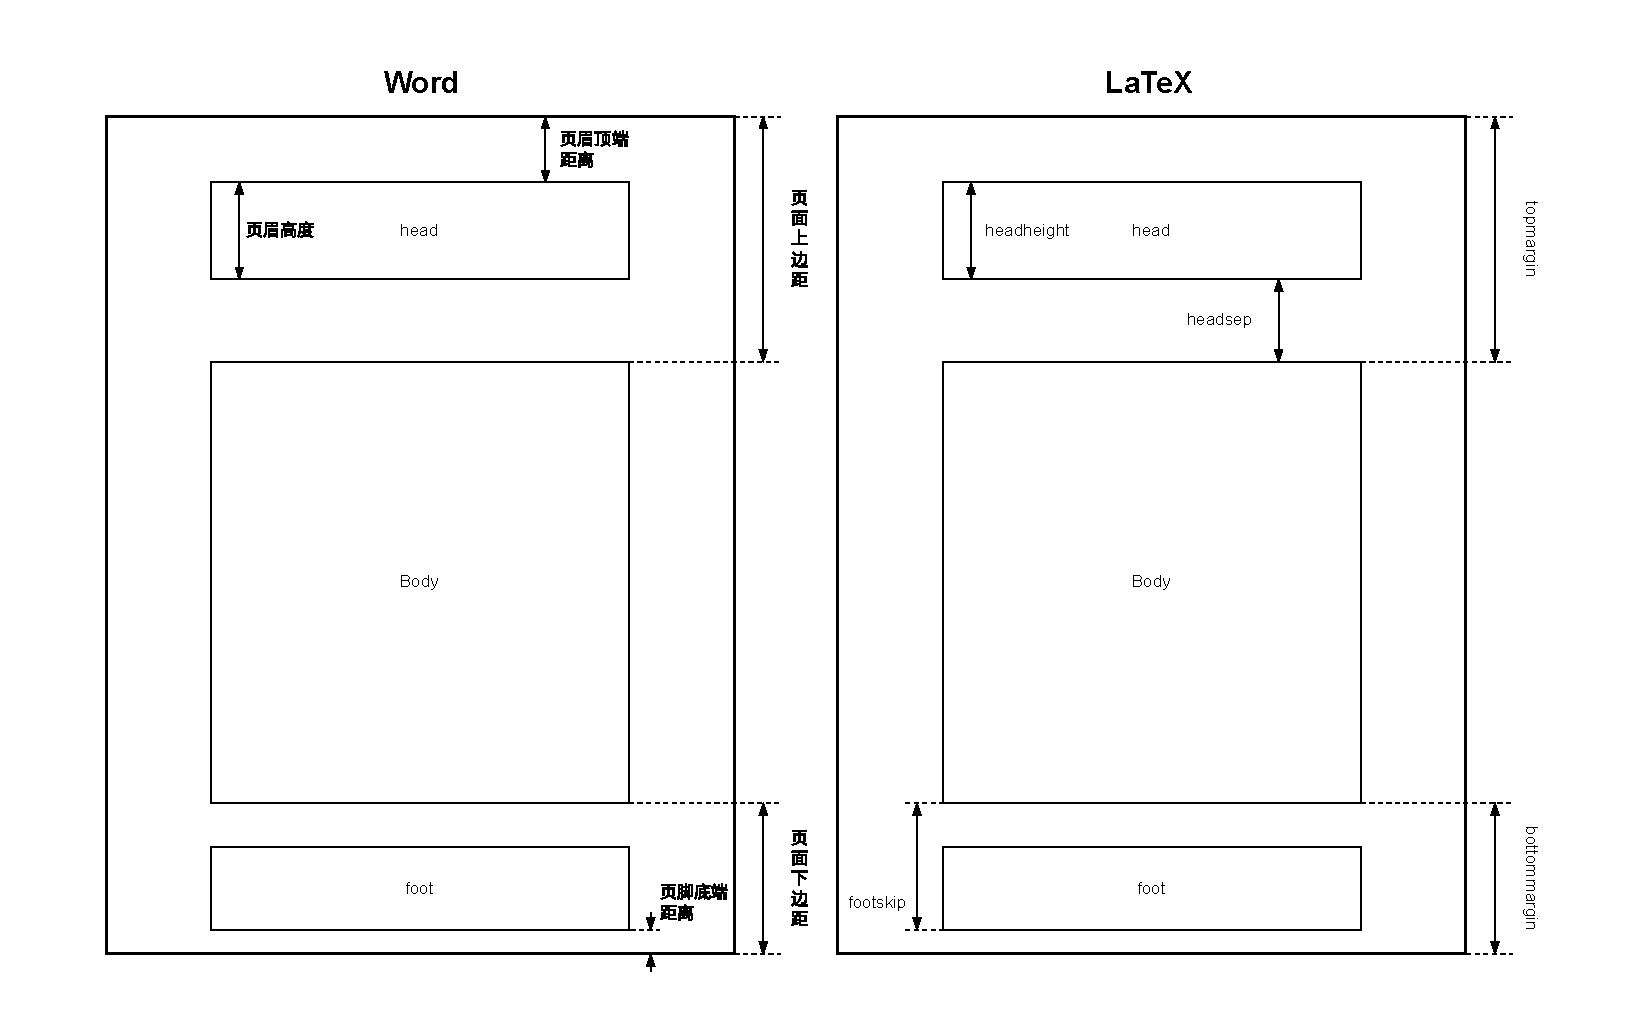
\includegraphics[width=0.9\linewidth]{figures/fig-headfoot.pdf}
%   \caption{Word 与 \LaTeX{} 页眉页脚度量基准对照}
%   \label{fig:headfoot-metrics}
% \end{figure}
% 
%    \begin{macrocode}
\RequirePackage{geometry}

\geometry{
	showframe=false,         % 显示排版边框
	verbose=true,           % 显示调试信息
	a4paper,                % A4（210mm × 297mm）
	includeheadfoot=false,  % 页眉页脚不计入版心
	bindingoffset=0.9cm,    % 装订线宽度
	left=2.5cm,             % 左边距
	right=2cm,              % 右边距
	top=2.74cm,             % 上边距
	bottom=2.2cm,           % 下边距
	headheight=0.7cm,       % 页眉区域高度
	headsep=8bp,            % 页眉下边界到版心上边界的距离
	footskip=0.45cm,        % 版心下边界到页脚基线的距离
}
%    \end{macrocode}
%    
% \subsection{字体与段落}
% 
% \subsubsection{字体集}
% 
% 定义七个中文字体切换命令，供正文中随时调用。
% 
%    \begin{macrocode}
\newcommand\songti  {\CJKfamily{zhsong}}
\newcommand\heiti   {\CJKfamily{zhhei}}
\newcommand\kaishu  {\CJKfamily{zhkai}}
\newcommand\fangsong{\CJKfamily{zhfs}}
\newcommand\lishu   {\CJKfamily{zhli}}
%    \end{macrocode}
%
%    \begin{macrocode}
\newcommand\hau@set@fonts@none{}
%    \end{macrocode}
%    
% 字体集简易自动检测
% 
%    \begin{macrocode}
\newcommand\hau@set@fonts@auto{%
	\IfFontExistsTF{SimSun}%
		{\hau@set@fonts@windows}%
		{\IfFontExistsTF{Songti SC}%
			 {\hau@set@fonts@macos}%
			 {\hau@set@fonts@linux}}%
}
%    \end{macrocode}
%    
%    Windows 字体集
%    
%    \begin{macrocode}
\newcommand\hau@set@fonts@windows{%
	\IfFontExistsTF{SimSun}
		{%
			\setmainfont{Times New Roman}%
			\setCJKmainfont{SimSun}[AutoFakeBold=2, AutoFakeSlant=0.2]%
			\setCJKfamilyfont{zhsong}{SimSun}[AutoFakeBold=2, AutoFakeSlant=0.2]%
			\setCJKfamilyfont{zhhei}{SimHei}[AutoFakeBold=2, AutoFakeSlant=0.2]%
			\setCJKfamilyfont{zhkai}{KaiTi}[AutoFakeBold=2, AutoFakeSlant=0.2]%
			\setCJKfamilyfont{zhfs}{FangSong}[AutoFakeBold=2]%
			\setCJKfamilyfont{zhli}{LiSu}[AutoFakeBold=2]%
			\newCJKfontfamily{\bfkai}{KaiTi}[FakeBold=2]%
		}%
		{%
			\PackageWarning{hauthesis}{'windows' fonts not found; switching to 'auto'}%
			\hau@set@fonts@auto
		}%
}
%    \end{macrocode}
%    
%    MacOS 字体集
%    
%    \begin{macrocode}
\newcommand\hau@set@fonts@macos{%
	\IfFontExistsTF{Songti SC}
		{%
			\setmainfont{Times New Roman}%
			\setCJKmainfont{Songti SC}[AutoFakeBold=2, AutoFakeSlant=0.2]%
			\setCJKfamilyfont{zhsong}{Songti SC}[AutoFakeBold=2, AutoFakeSlant=0.2]%
			\setCJKfamilyfont{zhhei}{Heiti SC}[AutoFakeBold=2, AutoFakeSlant=0.2]%
			\setCJKfamilyfont{zhkai}{Kaiti SC}[AutoFakeBold=2, AutoFakeSlant=0.2]%
			\setCJKfamilyfont{zhfs}{STFangsong}[AutoFakeBold=2]%
			\setCJKfamilyfont{zhli}{STLiti}[AutoFakeBold=2]%
			\newCJKfontfamily{\bfkai}{Kaiti SC}[FakeBold=2]%
		}%
		{%
			\PackageWarning{hauthesis}{'macos' fonts not found; switching to 'auto'}%
			\hau@set@fonts@auto
		}%
}
%    \end{macrocode}
%    
%    Linux 字体集
%    
%    \begin{macrocode}
\newcommand\hau@set@fonts@linux{%
	\IfFontExistsTF{FandolSong-Regular.otf}
		{%
			\setmainfont{texgyretermes}[%
				Extension      = .otf,%
				UprightFont    = *-regular,%
				BoldFont       = *-bold,%
				ItalicFont     = *-italic,%
				BoldItalicFont = *-bolditalic,%
			]%
			\setCJKmainfont{FandolSong-Regular.otf}[AutoFakeBold=2, AutoFakeSlant=0.2]%
			\setCJKfamilyfont{zhsong}{FandolSong-Regular.otf}[AutoFakeBold=2, AutoFakeSlant=0.2]%
			\setCJKfamilyfont{zhhei}{FandolHei-Regular.otf}[AutoFakeBold=2, AutoFakeSlant=0.2]%
			\setCJKfamilyfont{zhkai}{FandolKai-Regular.otf}[AutoFakeBold=2, AutoFakeSlant=0.2]%
			\setCJKfamilyfont{zhfs}{FandolFang-Regular.otf}[AutoFakeBold=2]%
			\setCJKfamilyfont{zhli}{FandolKai-Regular.otf}[AutoFakeBold=2]%
			\newCJKfontfamily{\bfkai}{FandolKai-Regular.otf}[FakeBold=2]%
		}%
		{%
			\PackageError{hauthesis}{No usable CJK fonts found}{%
				Install Fandol fonts (they ship with TeX Live), or pass [none] and set fonts yourself.}%
		}%
}
%    \end{macrocode}
%    
%    选择 字体集
%    
%    \begin{macrocode}
\@ifundefined{hau@set@fonts@\hau@fontset}%
	{\PackageError{hauthesis}{Unknown fontset '\hau@fontset'}{}}%
	{\expandafter\let\expandafter\hau@set@fonts
		 \csname hau@set@fonts@\hau@fontset\endcsname}%
\hau@set@fonts
%    \end{macrocode}
% 
% \subsubsection{字号与段落间距}
% 
% \entry{声明}
% 本节所有内容说明以及图表均参考自 \pkg{zhlineskip} 宏包说明文档。
% 
% 西文排版里，相邻两行基线（baseline）之间的距离称为行距（leading）。
% 西文字母四周与字框之间空隙较大，因此行距通常为字号的 1.2 至 1.45 倍。
% 
% \begin{figure}[htbp]
%   \centering
%   
\includegraphics[width=0.9\linewidth,page=1]{figures/fig-metrics}
%   \caption{西文字体。绿色方框即为 em-box，它在纸上的实际边长就是西文字号}
%   \label{fig:latinmetrics}
% \end{figure}
% 
% 中文排版没有基线概念，对应的是底线（ideographic baseline）。
% 相邻两行底线之间的距离与西文行距等价；
% 而上一行底线到下一行顶线之间的距离称为行间距（linegap）。
% 汉字字面几乎占满字框，
% 因此需要更大的行间距 —— 中文书刊的行距一般为字号的 1.5 至 1.67 倍。
% 
% \begin{figure}[htbp]
%   \centering
%   
\includegraphics[width=0.7\linewidth,page=2]{figures/fig-metrics}
%   \caption{中文字体。汉字字面几乎占满整个字框，字框的边长即为中文字号}
%   \label{fig:cjkmetrics}
% \end{figure}
% 
% Microsoft Word 的“单倍行距”由字体的上伸部、
% 下伸部与行间隙共同决定，因此同一个字号在不同字体下，
% 单倍行距并不相同。
% 
% \begin{table}[htbp]
%   \centering
%   \caption{Microsoft Word 中「单倍行距」的值取决于字体}
%   \label{tab:wordsinglespace}
%   \begin{tabular}{ll}
%     \toprule
%     字体名称 & 「单倍行距」$\div$ 字号 \\
%     \midrule
%     Arial                            & 2355/2048 = 1.14990234375 \\
%     Times New Roman                  & 2355/2048 = 1.14990234375 \\
%     中易系列（宋体、黑体、楷体、仿宋）  & 332/256 = 1.296875 \\
%     华文中宋（Windows）               & 1479/1000 = 1.479 \\
%     微软雅黑 Light（Windows）         & 3400/2048 = 1.66015625 \\
%     微软雅黑 Regular/Bold            & 3513/2048 = 1.71533203125 \\
%     华文中宋（macOS）                 & 1723/1000 = 1.723 \\
%     微软雅黑 Light（macOS）           & 3542/2048 = 1.7294921875 \\
%     苹方（macOS）                     & 1820/1000 = 1.82 \\
%     思源宋体 1.001                    & 1869/1000 = 1.869 \\
%     思源黑体 2.000                    & 1882/1000 = 1.882 \\
%     思源黑体 1.004                    & 1924/1000 = 1.924 \\
%     \bottomrule
%   \end{tabular}
%   \par\smallskip
%   \footnotesize 数据来源：\pkg{zhlineskip} 宏包说明文档表 2。
% \end{table}
% 
% 学校提供的模板里，正文要求小四号宋体、1.5 倍行距，首行缩进两个汉字
% （并且在模板段落格式可以观察到段前 0 磅、段后 8 磅），
% 正文使用中易系列字体，其单倍行距为字号的 1.296875 倍，
% 故目标行距为 1.296875 $\times$ 1.5 = 1.9453125 倍字号，
% 而本模板取 1.2 $\times$ 1.625 = 1.95 倍字号，
% 相对误差 0.24\%（12bp 字号下为 23.4bp 对 23.34bp）
% 
% 在 LaTeX 中，基础行距由 \cs{fontsize} 的第二个参数给出：
% 
%    \begin{macrocode}
\renewcommand{\normalsize}{\fontsize{12bp}{14.4bp}\selectfont}
\linespread{1.625}

\setlength{\parindent}{2\ccwd}
\setlength{\parskip}{0bp}
\raggedbottom %\flushbottom
%    \end{macrocode}
%    
% 其中 14.4bp = 12bp × 1.2，
% 即基础行距为字号的 1.2 倍。
% 而 \cs{linespread} 乘的是基础行距，不是字号；
% 段后 8 磅来自学校模板 Word文件。\cs{raggedbottom} 允许各页高度不一致，
% 避免 \LaTeX{} 为了凑满整页而拉伸段落间距；
% 注释掉的 \cs{flushbottom} 是相反的选择。
% 
% \begin{table}[htbp]
%   \centering
%   \caption{各文档类选项设置的基础行距倍数}
%   \label{tab:baseskip}
%   \begin{tabular}{lcc}
%     \toprule
%     文档类选项 & 正文基础行距 & 脚注基础行距 \\
%     \midrule
%     \option{zihao=5}  & 1.2        & 1.2   \\
%     \option{zihao=-4} & 1.2        & 1.2   \\
%     \option{10pt}     & 12/10      & 9.5/8 \\
%     \option{11pt}     & 13.6/10.95 & 11/9  \\
%     \option{12pt}     & 14.5/12    & 12/10 \\
%     \bottomrule
%   \end{tabular}
%   \par\smallskip
%   \footnotesize 数据来源：\pkg{zhlineskip} 宏包说明文档表 1。
% \end{table}
% 
% \paragraph{为什么不用 \pkg{zhlineskip}}
% 
% \pkg{zhlineskip} 宏包正是为解决中西文混排的行距差异而作，
% 并提供了两个与本模板需求直接对口的选项：
% \option{MSWordLineSpacingMultiple} 与 \option{restoremathleading}。
% 本模板不引入它，有两个原因。
% 
% 第一，它对 \LaTeX{} 内核的要求过新。
% 宏包声明 \cs{NeedsTeXFormat}\{LaTeX2e\}[2026/06/01]，
% 即内核不早于 2026 年 6 月 1 日才能加载；
% 它还用到 \cs{ProcessKeyOptions} 这类较新的 \pkg{expl3} 接口。
% TeX Live 按年发行，因此实际上只有 \textbf{TeX Live 2026 及更新}的发行版可用。
% 本模板当前正是在 TeX Live 2026 上编译的，
% 其内核日期 \texttt{2026-06-01} 恰好是该宏包的下限，
% 较早的发行版（如 TeX Live 2025）若想使用该宏包，
% 若确需该宏包，须先升级发行版。
% 
% 第二，它会重新计算全文的竖直间距。
% 本模板的段后 8 磅、图表浮动间距、公式上下间距都是逐项测量调校的结果，
% 替换行距模型等于把它们全部重做。
% 
% \paragraph{代价}
% 
% 扩大全文行距会一并放大数学公式的行距。
% 数学公式主要由西文字符构成，按中文行距排版会显得松散。
% 本模板在需要紧凑行距的位置就地指定：
% 
% \begin{table}[htbp]
%   \centering
%   \caption{行距放大的影响与处理办法}
%   \label{tab:mathleading}
%   \begin{tabular}{ll}
%     \toprule
%     位置 & 做法 \\
%     \midrule
%     注释条目     & \cs{linespread}\{1\} 后接 \cs{fontsize}\{12pt\}\{18pt\} \\
%     英文摘要标题 & 用 \cs{rule}\{0pt\}\{\cs{hautitleline}\} 固定行高 \\
%     图表标题     & \cs{DeclareCaptionFont} 内前置 \cs{linespread}\{1\} \\
%     行间公式     & 多行数学环境统一恢复西文行距，见\ref{sec:mathenv}节 \\
%     \bottomrule
%   \end{tabular}
% \end{table}
% 
% 在 Word 中，段落文字的实际除了字号、基础行距、多倍行距之外，
% 还手段前段后间距的影响。
% \begin{figure}[htbp]
%   \centering
%   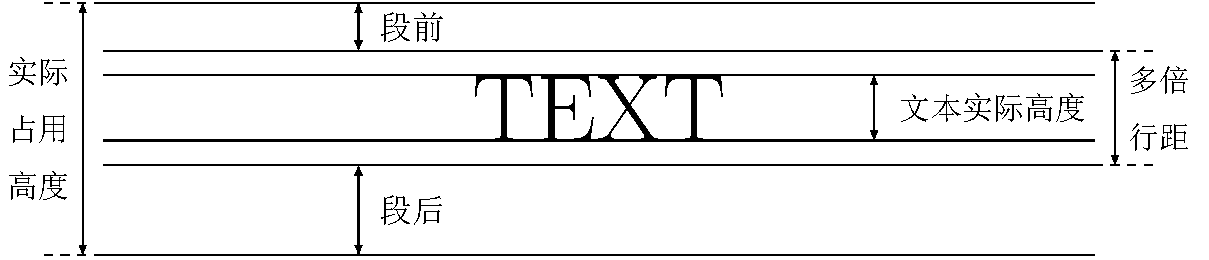
\includegraphics[width=0.9\linewidth]{figures/text.pdf}
%   \caption{Word 中字体行高}
%   \label{fig:text}
% \end{figure}
% 
% 最后要注意，学校规范中正文写作「1.5 倍行距」，
% 而注释写作「行距 18 磅」，这两者不是同一套换算：
% 
% \begin{table}[htbp]
%   \centering
%   \caption{规范中两处行距要求的换算}
%   \label{tab:leadingcompare}
%   \begin{tabular}{llll}
%     \toprule
%     位置 & 规范原文 & 换算 & 12bp 下 \\
%     \midrule
%     正文 & 1.5 倍行距 & Word 单倍 $\times$ 1.5 = 1.945 $\times$ 字号 & 23.4bp \\
%     注释 & 行距 18 磅 & 1.5 $\times$ 字号 & 18bp \\
%     \bottomrule
%   \end{tabular}
% \end{table}
% 
% 因此模板中注释用 \cs{fontsize}\{12pt\}\{18pt\}，正文用 \cs{linespread}\{1.625\}。
% 两者不是笔误，而是两条不同的规定。
% 
% \subsection{标题层级}
% \label{sec:headings}
% 
% \DescribeMacro{\chapter}
% \DescribeMacro{\section}
% \DescribeMacro{\subsection}
% 标题一共三个级别（章、节、条），分别对应
% \cs{chapter}、\cs{section}、\cs{subsection}。
% 在 Word 中，一级标题（章）为小三号黑体，加粗，段前 0.5 行，
% 段后 0.5 行，1.5 倍数行距；二级标题（节）为四号黑体，
% 加粗，段前 0 磅，段后 8 磅，1.5 倍行距；
% 三级标题（条）为小四号黑体，不加粗，段前 0 磅，
% 段后 8 磅，1.5倍啊行距。
% 
%    \begin{macrocode}
\renewcommand\chapter{%
	%\par\penalty-\@highpenalty
	\global\@topnum\z@
	\@afterindenttrue
	\secdef\@chapter\@schapter}

\ctexset{
	chapter = {
		name       = {},
		number     = \arabic{chapter},
		format     = \heiti\bfseries\zihao{-3},
		aftername  = \hspace{1\ccwd},
		fixskip    = true,
		beforeskip = 22.5bp,
		afterskip  = 22.5bp,
	},
	section = {
		format    = \heiti\bfseries\zihao{4},
		aftername = \hspace{1\ccwd},
		beforeskip = .2\baselineskip,
		afterskip  = .2\baselineskip,
	},
	subsection = {
		format    = \heiti\zihao{-4},
		aftername = \hspace{1\ccwd},
		beforeskip = .2\baselineskip,
		afterskip  = .2\baselineskip,
	},
}
%    \end{macrocode}
%  
% \subsection{页眉页脚与页码}
% 
%    \begin{macrocode}
\RequirePackage{fancyhdr}
\RequirePackage{lastpage}

\pagestyle{fancy}
\fancyhf{}
\newcommand{\hautotalpages}{\pageref{LastPage}}

\let\haudefaultCJKglue\CJKglue
\newcommand{\hauheaderspace}{%
	\xeCJKsetup{CJKglue={\haudefaultCJKglue\hskip 3pt}}%
}

\fancyhead[L]{{\bfseries\zihao{-2}\hauheaderspace \ 淮安大学毕业设计（论文）}}
\fancyhead[R]{\songti\zihao{-4}第 \thepage 页\quad 共 \hautotalpages 页}
\renewcommand{\headrulewidth}{0.5pt}
%    \end{macrocode}
% 
% \subsection{封面}
% 
% \entry{封面}
% 封面信息一律采用三号楷体、Times New Roman，居中排版。封面信息包括：学校名称、论文类型、学生姓名、学号、学院、专业、论文题目、指导教师姓名及职称、论文提交日期。
% 
%    \begin{macrocode}
\RequirePackage{tabularray}
\RequirePackage{graphicx}

\def\YourName{}
\def\YourNumber{}
\def\YourCollege{}
\def\YourMajor{}
\def\PaperTitleLa{}
\def\PaperTitleLb{}
\def\SupervisorNameIn{}
\def\SupervisorTitleIn{}
\def\SupervisorNameOut{}
\def\SupervisorTitleOut{}
\def\PaperYear{}
\def\PaperMonth{}
\def\PaperTitleENa{}
\def\PaperTitleENb{}
\def\Keywords{}
\def\KeywordsEN{}

\newcommand{\MakeCover}{%
	\vspace*{2\baselineskip}%
	\thispagestyle{empty}%
	\begin{center}%
		{\kaishu\fontsize{26pt}{32.5pt}\selectfont 淮 \ 安 \ 大 \ 学}\\[5.5em]
		{\heiti\fontsize{38pt}{47.5pt}\selectfont 毕业设计（论文）}\\[7.5em]
		\kaishu\zihao{3}%
		\begin{tblr}{
				colspec = {Q[b,j,wd=2.9cm]Q[b,c,wd=0.9cm]Q[b,c,wd=2.1cm]Q[b,c,wd=1.4cm]
									 Q[b,c,wd=0.6cm]Q[b,c,wd=2.9cm]Q[b,c,wd=0.9cm]},
				colsep = 6pt,
				row{1-Z} = {ht=1cm, abovesep=10pt, belowsep=0pt},
				hspan = minimal, vspan = minimal,
			}
			\bfkai 学 \ 生 \ 姓 \ 名： & \SetCell[c=2]{b,c}\YourName &&
				\SetCell[c=2]{b,c}\bfkai 学\hspace{1em}号： &&
				\SetCell[c=2]{b,c}\YourNumber & \\
			\cline{2-3}\cline{6-7}
			\bfkai 学\hspace{2.7em}院： & \SetCell[c=6]{b,c}\YourCollege &&&&&& \\
			\cline{2-7}
			\bfkai 专\hspace{2.7em}业： & \SetCell[c=6]{b,c}\YourMajor &&&&&& \\
			\cline{2-7}
			\bfkai\scalebox{0.6}[1]{设计（论文）题目}： &
				\SetCell[c=6]{b,c}\PaperTitleLa &&&&&& \\
			\cline{2-7}
			\rule{0pt}{20pt} & \SetCell[c=6]{b,c}\PaperTitleLb &&&&&& \\
			\cline{2-7}
			\bfkai\scalebox{0.8}[1]{校内指导老师}： &&
				\SetCell[c=2]{b,c}\SupervisorNameIn &&
				\SetCell[c=2]{b,c}\SupervisorTitleIn &&\\
			\cline{2-7}
			\bfkai\scalebox{0.8}[1]{校外指导老师}： &&
				\SetCell[c=2]{b,c}\SupervisorNameOut &&
				\SetCell[c=2]{b,c}\SupervisorTitleOut &&\\
			\cline{2-7}
		\end{tblr}%
		\par\vspace{6em}%
		{\heiti\fontsize{16pt}{20pt}\selectfont
			\PaperYear\hspace{1em}年\hspace{1em}\PaperMonth\hspace{1em}月}%
	\end{center}%
}
%    \end{macrocode}
% 
% \subsection{摘要}
% 
% 摘要分中文与外文两部分，两者都不编号、各自另起一页，
% 标题（页眉）字体为三号宋体，居中，适当拉宽。
% 
% 整页的版式交给 \env{hauabstractpage} 环境处理：
% 它负责换页、重设页边距、切换页眉样式，
% 并把整页内容装进一个带外框的 \env{minipage} 中，
% 中英文摘要页的外框尺寸与位置完全一致。
% 
%    \begin{macrocode}
\newcommand{\abstracthead}{}
\newsavebox{\abstractbox}

\fancypagestyle{hauabstract}{%
	\fancyhf{}%
	\fancyhead[C]{{\zihao{3}\hauheaderspace\abstracthead}}%
	\renewcommand{\headrulewidth}{0pt}%
}

\newenvironment{hauabstractpage}[1]{%
	\renewcommand{\abstracthead}{#1}%
	\clearpage
	\newgeometry{
		showframe=false,        % 显示排版边框
		includeheadfoot=false,  % 页眉页脚不计入版心
		bindingoffset=0.9cm,    % 装订线宽度
		left=2.5cm,             % 左边距
		right=2cm,              % 右边距
		top=2.74cm,             % 上边距
		bottom=2.2cm,           % 下边距
		headheight=0.7cm,       % 页眉区域高度
		headsep=0.25cm,         % 页眉下边界到版心上边界的距离
		footskip=0.45cm,        % 版心下边界到页脚基线的距离
	}%
	\thispagestyle{hauabstract}%
	\setlength{\fboxsep}{0.5em}%
	\setlength{\fboxrule}{1bp}%
	\begin{lrbox}{\abstractbox}%
		\begin{minipage}[c][\dimexpr\textheight-2\fboxsep-2\fboxrule][t]%
										{\dimexpr\textwidth-2\fboxsep-2\fboxrule}%
			\songti\zihao{-4}%
}{%
		\end{minipage}%
	\end{lrbox}%
	\noindent\fbox{\usebox{\abstractbox}}%
	\clearpage
	\restoregeometry
}
%    \end{macrocode}
% 
% \subsubsection{中文摘要}
% 
% \DescribeEnv{cnabstract}
% 中文摘要使用 \env{cnabstract} 环境，
% 正文为小四号宋体，首行缩进两个汉字。
% 关键词在摘要末尾间隔两行另起一行，
% 以「关键词」三字起头，“关键词”为小四号加粗黑体，
% 并用 2 个空格隔开，后面关键词使用全角都好“，”隔开，
% 最后一个关键词后面不加逗号。
% 
%    \begin{macrocode}

\newcommand{\keywordsCN}[1]{%
	\par\vspace{2\baselineskip}\noindent
	{\heiti 关键词}\hspace{1\ccwd}#1\par
}
\newenvironment{cnabstract}%
	{\begin{hauabstractpage}{毕业设计（论文）中文摘要}%
	 \vspace*{\baselineskip}% 先空一行
	 \parindent=2\ccwd}%      每段首行缩进两个汉字
	{\keywordsCN{\Keywords}%
	 \end{hauabstractpage}}
%    \end{macrocode}
% 
% \subsubsection{英文摘要}
% 
% \DescribeEnv{enabstract}
% 英文摘要使用 \env{enabstract} 环境。
% 标题块由 \cs{hauabstracttitle} 排版：
% 左侧固定放 \textbf{Title} 标签（三号），
% 右侧两行分别是英文题名（四号）的第一行与第二行，
% 每行下方各有一条横线；两行的行高由 \cs{hautitleline} 统一控制。
% 标题块之后是空一行是 \textbf{Abstract} 标签与摘要正文。
% 
% 英文摘要正文的行距比中文摘要紧凑（\cs{linespread}\{1.2\}），
% 因为西文按排版惯例不需要中文那么大的行间距。关键词以
% \textbf{Keywords} 起头，格式与中文摘要的关键词对应（逗号为半角逗号“,”）。
% 
%    \begin{macrocode}
\newlength{\hautitlelabelwd}
\newlength{\hautitletextwd}
\newlength{\hautitleline}

% 行高 = 三号 16bp × 1.3 × 1.5= 31.2bp
\setlength{\hautitleline}{31.2bp}

\newcommand{\hauabstracttitle}[2]{%
	\begingroup
	\parskip=0pt
	\par\noindent
		\settowidth{\hautitlelabelwd}{\zihao{3}\bfseries Title\hspace{0.5em}}%
		\setlength{\hautitletextwd}{\dimexpr\linewidth-\hautitlelabelwd\relax}%
		\begin{tabular}{@{}l@{}p{\hautitletextwd}@{}}
			\noindent\rule[-6bp]{0pt}{\hautitleline}\zihao{3}\bfseries Title\hspace{0.5em} &
			\noindent\rule[-6bp]{0pt}{\hautitleline}\makebox[\hautitletextwd][c]{\zihao{4}#1} \\ \cline{2-2}
			\noalign{\vskip 26.4bp}%
			\noindent\rule[-6bp]{0pt}{\hautitleline} &
			\noindent\rule[-6bp]{0pt}{\hautitleline}\makebox[\hautitletextwd][c]{\zihao{4}#2} \\ \cline{2-2}
		\end{tabular}%
	\par\vspace{26bp}%
	\noindent{\zihao{3}\bfseries\rule{0pt}{\hautitleline}Abstract}\par
	\vspace{23.2bp}%
	\endgroup
}

\newcommand{\keywordsEN}[1]{%
	\par\vspace{2\baselineskip}%
	{\bfseries Keywords}\hspace{1\ccwd}#1\par
}

\newenvironment{enabstract}%
	{\begin{hauabstractpage}{毕业设计（论文）外文摘要}%
	 \hauabstracttitle{\PaperTitleENa}{\PaperTitleENb}%
	 \linespread{1.2}\selectfont}%
	{\keywordsEN{\KeywordsEN}%
	 \end{hauabstractpage}}
%    \end{macrocode}
% 
% \subsection{目录}
% \DescribeEnv{hautocstart}
% \DescribeEnv{hautocend}
% 目录采用 \cs{hautocstart} 和 \cs{hautocend} 控制，
% 标题为“目\hspace{1.5em}录”（之间三个空格），
% 居中，三号黑体，接着空一行（四行的 Word 参数为宋体，
% 四号，1.5 倍行距，段前 0 磅，段后 8 磅），
% 然后开始目录条目：小四号宋体，固定行距 18 磅
% （每个条目为一个段落，注意叠加上段后 8 磅，即 18 + 8 = 26 磅），
% 编号到三级标题，编号与标题之间一个空格，
% 目录条目与页码之间用点线连接，页码右对齐。
% 
%    \begin{macrocode}
\newcommand{\hautocstart}{%
	\clearpage
	\pagenumbering{Roman}%
	\renewcommand{\hautotalpages}{\pageref{hauctocend}}%
	\pagestyle{fancy}%
}

\newcommand{\hautocend}{%
	\label{hauctocend}%
	\clearpage
	\renewcommand{\hautotalpages}{\pageref{LastPage}}%
}

\renewcommand{\tableofcontents}{%
	\clearpage
	\begingroup
	\parskip=0pt \topsep=0pt \partopsep=0pt
	\vspace*{70.6bp}%
	\begin{center}%
		{\linespread{1}\heiti\fontsize{14pt}{21pt}\selectfont 目\hspace{1.5em}录}%
	\end{center}%
	\vspace*{43.3bp}%
		\linespread{1}\songti\fontsize{12bp}{26bp}\selectfont
		\@starttoc{toc}%
	\endgroup
}

\renewcommand{\@dotsep}{2.5}
\renewcommand*\l@chapter{\@dottedtocline{0}{0em}{1.0em}}
\renewcommand*\l@section{\@dottedtocline{1}{0em}{2.0em}}
\renewcommand*\l@subsection{\@dottedtocline{2}{0em}{2.8em}}
\renewcommand*\l@subsubsection{\@dottedtocline{3}{0em}{4.0em}}
%    \end{macrocode}
%
% 不编号的章（总结与展望、致谢、注释、参考文献）：缩进与编号宽度都为零，目录里顶格：
% 
%    \begin{macrocode}
\newcommand*\l@unnumbered{\@dottedtocline{0}{0em}{0em}}
%    \end{macrocode}
% 
% \subsection{图表}
% 
% \entry{figures \& table}
% 加载图片路径
% 
%    \begin{macrocode}
\graphicspath{{figures/}}
%    \end{macrocode}
% 
% 图表可以通过参数选择是否包含章节号，默认包含。
% 
%    \begin{macrocode}
\RequirePackage{caption}

\ifhau@num@fig
  \counterwithin{figure}{chapter}
  \renewcommand{\thefigure}{\thechapter-\arabic{figure}}
\else
  \counterwithout{figure}{chapter}
  \renewcommand{\thefigure}{\arabic{figure}}
\fi
\ifhau@num@tab
  \counterwithin{table}{chapter}
  \renewcommand{\thetable}{\thechapter-\arabic{table}}
\else
  \counterwithout{table}{chapter}
  \renewcommand{\thetable}{\arabic{table}}
\fi
%    \end{macrocode}
%    
% 标题样式
%    
%    \begin{macrocode}
\DeclareCaptionLabelFormat{haucapfmt}{#1#2}
\DeclareCaptionLabelSeparator{haucapsep}{\hspace{1\ccwd}}
\DeclareCaptionFont{haucapfont}{\linespread{1}\songti\fontsize{10.5pt}{12.6pt}\selectfont}
\captionsetup{
	font          = haucapfont,
	labelformat   = haucapfmt,
	labelsep      = haucapsep,
	justification = centering,
}
\captionsetup[table]{position=top}
\captionsetup[figure]{position=bottom}
%    \end{macrocode}
%    
%    段落间距
% 
%    \begin{macrocode}
\setlength{\textfloatsep}{12pt plus 2pt minus 2pt}   % 浮动体在页顶/页底时
\setlength{\intextsep}{12pt plus 2pt minus 2pt}      % 浮动体夹在正文中间时
\setlength{\floatsep}{12pt plus 2pt minus 2pt}       % 两个浮动体之间

\captionsetup[table]{skip=6pt, aboveskip=6pt}   % 表题：与表格之间 6pt，上方 6pt
\captionsetup[figure]{skip=6pt, belowskip=6pt}  % 图题：与图片之间 6pt，下方 6pt

\g@addto@macro\@floatboxreset{%
	\linespread{1}%
	\songti\fontsize{10.5pt}{12.6pt}\selectfont
	\renewcommand\arraystretch{1.35}%
}
%    \end{macrocode}
% 
% \subsection{列表环境}
% 
% 正文里的无序列表（\env{itemize}）、有序列表（\env{enumerate}）与描述列表
% （\env{description}）由 \pkg{enumitem} 宏包排版。
% 
% 标准文档类为列表预设了一组间距：列表与上下文的 \cs{topsep}（8\,pt）、
% 列表作为新段落开头时额外附加的 \cs{partopsep}（2\,pt）、条目之间的
% \cs{itemsep}（4\,pt），以及条目内段落之间的 \cs{parsep}（4\,pt）。
% 本模板的正文段间距为 0，若沿用这些默认值，列表会显得格外松散。
% 
% 因此在加载宏包之后统一归零，让列表与正文的间距保持一致：
% 
%    \begin{macrocode}
\RequirePackage{enumitem}

\setlist{
	topsep    = 0pt,
	partopsep = 0pt,
	parsep    = 0pt,
	itemsep   = 0pt,
}
%    \end{macrocode}
% 
% \subsection{数学环境}\label{sec:mathenv}
% 
% \subsubsection{数学字体}
% 
% \entry{TeX Gyre Termes}
% 数学环境下的字体使用 TeX Gyre Termes。
% 
%    \begin{macrocode}
\RequirePackage{unicode-math}
\setmathfont{texgyretermes-math.otf}

% 多行公式、矩阵、cases 等环境内部恢复西文行距。
% 否则 \linespread{1.625} 给出的 23.4pt 行距会一并放大公式的行间
% （amsmath 的多行环境以 \baselineskip 为行间基准）。
\RequirePackage{etoolbox}
\newcommand{\hau@mathleading}{\linespread{1}\selectfont}
\newcommand{\hau@setmathleading}[1]{%
	\AtBeginEnvironment{#1}{\hau@mathleading}}
\forcsvlist{\hau@setmathleading}{%
	align,align*,alignat,alignat*,flalign,flalign*,
	gather,gather*,multline,multline*,
	split,aligned,alignedat,gathered,
	array,matrix,pmatrix,bmatrix,Bmatrix,vmatrix,Vmatrix,cases,dcases}
%    \end{macrocode}
% 
% \subsubsection{公式段落编号}
% 
%    \begin{macrocode}
\ifhau@num@eqn
  \counterwithin{equation}{chapter}
  \renewcommand{\theequation}{\thechapter-\arabic{equation}}
\else
  \counterwithout{equation}{chapter}
  \renewcommand{\theequation}{\arabic{equation}}
\fi

\setlength{\abovedisplayskip}{10pt plus 2pt minus 5pt}
\setlength{\belowdisplayskip}{10pt plus 2pt minus 5pt}
\setlength{\abovedisplayshortskip}{0pt plus 3pt}
\setlength{\belowdisplayshortskip}{6pt plus 3pt minus 3pt}
% 多行公式（align/gather）两行之间的距离
\setlength{\jot}{6pt}
%    \end{macrocode}
% 
% \subsection{算法与伪代码}
% \label{sec:algorithm}
% 
% 伪代码用 \pkg{algorithm} 与 \pkg{algpseudocode} 两个宏包排版。前者提供
% 浮动体与编号，后者提供 \cs{State}、\cs{For}、\cs{If} 等语句。
% 
%    \begin{macrocode}
\RequirePackage{algorithm}
\RequirePackage{algpseudocode}
%    \end{macrocode}
% 
% 默认排出的是英文的「Algorithm 1」「Require:」，需要改成中文：
% 
%    \begin{macrocode}
\floatname{algorithm}{算法}
\renewcommand{\algorithmicrequire}{\textbf{输入：}}
\renewcommand{\algorithmicensure}{\textbf{输出：}}
\renewcommand{\algorithmiccomment}[1]{\hfill/* #1 */}
%    \end{macrocode}
% 
% 编号与图表公式一致，采用「算法 1-1」的形式：
% 
%    \begin{macrocode}
\ifhau@num@alg
  \counterwithin{algorithm}{chapter}
  \renewcommand{\thealgorithm}{\thechapter-\arabic{algorithm}}
\else
  \counterwithout{algorithm}{chapter}
  \renewcommand{\thealgorithm}{\arabic{algorithm}}
\fi
%    \end{macrocode}
% 
% 算法的正文与标题都用五号字，与图表一致。正文的字号在环境开始时统一设定，
% 上下留白的四处公式间距也一并收紧：
% 
%    \begin{macrocode}
\AtBeginEnvironment{algorithm}{%
  \fontsize{10.5pt}{12.6pt}\selectfont
  \setlength{\abovedisplayskip}{6pt plus 2pt minus 2pt}%
  \setlength{\belowdisplayskip}{6pt plus 2pt minus 2pt}%
  \setlength{\abovedisplayshortskip}{6pt plus 2pt minus 2pt}%
  \setlength{\belowdisplayshortskip}{6pt plus 2pt minus 2pt}%
}
%    \end{macrocode}
% 
% 标题归 \pkg{caption} 宏包管，需要先注册一个五号的字体设置再套用：
% 
%    \begin{macrocode}
\DeclareCaptionFont{hauwuhao}{\fontsize{10.5pt}{12.6pt}\selectfont}
\captionsetup[algorithm]{font={hauwuhao}}
%    \end{macrocode}
% 
% \env{algorithm} 是浮动体，位置由 \LaTeX{} 安排，因此一个算法不会被拆到
% 两页上；正文中需要用 \cs{ref} 指向它。
% 
% \subsection{总结与展望}
% 
% \DescribeEnv{conclusion}
% 总结与展望使用 \env{conclusion} 环境，开头空两行之后是标题，
% 为“总结与展望”，居中，小三号黑体，接着空一行（前四行的 Word 参数为宋体，
% 四号，1.5 倍行距，段前 0 磅，段后 8 磅），
% 然后开始正文：小四号宋体，1.5 倍行距，段前 0 磅，段后 8 磅。
%    \begin{macrocode}
\newenvironment{conclusion}{%
	\clearpage
	\begingroup
		\parskip=0pt \topsep=0pt \partopsep=0pt
		\vspace*{56.5bp}%
		\phantomsection
		\addcontentsline{toc}{unnumbered}{总结与展望}%
		\begin{center}%
			{\linespread{1}\heiti\fontsize{15bp}{22.5bp}\selectfont 总结与展望}%
		\end{center}%
		\vspace*{27.25bp}%
	\endgroup
}{%
	\clearpage
}
%    \end{macrocode}

% \subsection{致谢}
% 
% \DescribeEnv{acknowledgements}
% 致谢部分格式与总结与展望类似，
% “致谢”两个字之间两个空格。
% 
%    \begin{macrocode}
\newenvironment{acknowledgements}{%
	\clearpage
	\begingroup
		\parskip=0pt \topsep=0pt \partopsep=0pt
		\vspace*{56.5bp}%
		\phantomsection
		\addcontentsline{toc}{unnumbered}{致谢}%
		\begin{center}%
			{\linespread{1}\heiti\fontsize{15bp}{22.5bp}\selectfont 致 \quad 谢}%
		\end{center}%
		\vspace*{27.25bp}%
	\endgroup
}{%
	\clearpage
}
%    \end{macrocode}

% \subsection{注释}

%    \begin{macrocode}
% 注释列表的可调数值
\newlength{\hau@note@itemsep}
\newlength{\hau@note@line}
\setlength{\hau@note@itemsep}{6pt}
\setlength{\hau@note@line}{18pt}

\newcommand{\notemark}[1]{%
	\hyperlink{note@#1}{\textsuperscript{[#1]}}%
}

\newlist{notelist}{enumerate}{1}
\setlist[notelist]{%
	label       = [\arabic*],
	labelindent = 0pt,
	leftmargin  = *,
	labelsep    = 0.5em,
	widest      = 99,
	topsep      = 0pt,
	partopsep   = 0pt,
	parsep      = 0pt,
	itemsep     = \hau@note@itemsep,
	before      = \vspace{0pt},
	after       = \vspace{0pt},
}

\newenvironment{notes}{%
	\clearpage
	\begingroup
		\parskip=0pt \topsep=0pt \partopsep=0pt
		\vspace*{56.5bp}%
		\phantomsection
		\addcontentsline{toc}{unnumbered}{注释}%
		\begin{center}%
			{\linespread{1}\heiti\fontsize{15bp}{22.5bp}\selectfont 注 \quad 释}%
		\end{center}%
		\vspace*{27.25bp}%
	\endgroup
	\songti\linespread{1}\fontsize{12pt}{\hau@note@line}\selectfont
	\begin{notelist}%
	\let\hau@noteitem\item
	\renewcommand{\item}{\hau@noteitem\hypertarget{note@\arabic{notelisti}}{}}%
}{%
	\end{notelist}%
	\clearpage
}
%    \end{macrocode}
%    
% \subsection{参考文献}

% 标题区与「总结与展望」「致谢」完全一致：另起一页，空两行、标题居中、
% 空一行，四行均为小三号黑体、1.5 倍行距、段前 0 磅、段后 8 磅。
%
% 用哪种方案由用户加载的宏包决定，两种都自动识别，用户不需要设置任何选项：
%   biblatex        —— \cs{printbibliography}
%   BibTeX + natbib —— \cs{bibliography}
% 标题文字固定为「参考文献」，不接受 \cs{printbibliography} 的 title 选项覆盖。

%    \begin{macrocode}
\RequirePackage{filehook}
\RequirePackage{etoolbox}

% biblatex
\AtEndOfPackageFile*{biblatex}{
	\defbibheading{bibliography}[\bibname]{%
		\clearpage
		\begingroup
			\parskip=0pt \topsep=0pt \partopsep=0pt
			\vspace*{56.5bp}%
			\phantomsection
			\addcontentsline{toc}{unnumbered}{参考文献}%
			\begin{center}%
				{\linespread{1}\heiti\fontsize{15bp}{22.5bp}\selectfont 参\ 考\ 文\ 献}%
			\end{center}%
		\vspace*{19.25bp}%
		\endgroup
	}
	\renewcommand\bibfont{\linespread{1}\fontsize{12bp}{18bp}\selectfont}%
	\setlength{\bibitemsep}{0pt plus 2pt}%
	\setlength{\bibhang}{1cm}%
}

% BibTeX + natbib
\AtEndOfPackageFile*{natbib}{
	\patchcmd{\thebibliography}{\chapter*{\bibname}}{%
		\clearpage
		\begingroup
			\parskip=0pt \topsep=0pt \partopsep=0pt
			\vspace*{56.5bp}%
			\phantomsection
			\addcontentsline{toc}{unnumbered}{参考文献}%
			\begin{center}%
				{\linespread{1}\heiti\fontsize{15bp}{22.5bp}\selectfont 参\ 考\ 文\ 献}%
			\end{center}%
		\vspace*{19.25bp}%
		\endgroup
	}{}{\PackageError{hauthesis}{\string\thebibliography\space 的内部结构已变，标题补丁失败}{}}
	\renewcommand\bibfont{\linespread{1}\fontsize{12bp}{18bp}\selectfont}%
	\setlength{\bibsep}{0pt plus 2pt}%
	\setlength{\bibhang}{1cm}%
}
%    \end{macrocode}
% \subsection{附录}
% 附录章节标题采用默认格式。
% 
% \subsection{代码环境}
% \label{sec:code}
% 
% \subsubsection{代码字体}
% 
% 代码块的西文默认使用 Times New Roman 的 \TeX{} 替代字体
% TeX Gyre Termes，中文使用宋体 FandolSong，两者都随 \TeX{} Live 提供，
% 各平台一致，不受操作系统影响。
% 
% 另提供一个等宽组合 \cs{codeMono}：西文用 Consolas，中文用仿宋，
% 用于需要严格等宽对齐的代码。若系统中没有 Consolas，自动改用
% DejaVu Sans Mono。
% 
%    \begin{macrocode}
\RequirePackage{listings}
\RequirePackage{xcolor}

\IfFontExistsTF{TeX Gyre Termes}
  {\newfontfamily\codeLatin{TeX Gyre Termes}}
  {\newfontfamily\codeLatin{DejaVu Serif}}
\IfFontExistsTF{FandolSong-Regular.otf}
  {\setCJKfamilyfont{codeCJK}{FandolSong-Regular.otf}}
  {\setCJKfamilyfont{codeCJK}{SimSun}}
\IfFontExistsTF{Consolas}
  {\newfontfamily\codeMonoLatin{Consolas}}
  {\newfontfamily\codeMonoLatin{DejaVu Sans Mono}}
\IfFontExistsTF{FandolFang-Regular.otf}
  {\setCJKfamilyfont{codeMonoCJK}{FandolFang-Regular.otf}}
  {\setCJKfamilyfont{codeMonoCJK}{FangSong}}
\newcommand{\codeMono}{\CJKfamily{codeMonoCJK}\codeMonoLatin}
%    \end{macrocode}
% 
% \subsubsection{配色}
% 
% 配色做成具名的方案，用 \cs{hautocodestyle} 挑选，不写参数时用默认的
% 黑白方案。要新增一套方案，照下面的样子加一个 \cs{hau@codestyle@名字}
% 即可，其余部分不必改动。
% 
%    \begin{macrocode}
\newcommand{\hau@codestyle@black}{%
  \definecolor{hlkw}{RGB}{0, 0, 0}%
  \definecolor{hlcm}{RGB}{0, 0, 0}%
  \definecolor{hlstr}{RGB}{0, 0, 0}%
  \definecolor{codebg}{RGB}{255, 255, 255}%
  \definecolor{hlbasic}{RGB}{0, 0, 0}%
}
\newcommand{\hau@codestyle@vscode}{%
  \definecolor{hlkw}{RGB}{86, 156, 214}%
  \definecolor{hlcm}{RGB}{106, 153, 85}%
  \definecolor{hlstr}{RGB}{206, 145, 120}%
  \definecolor{codebg}{RGB}{255, 255, 255}%
  \definecolor{hlbasic}{RGB}{0, 0, 0}%
}
\newcommand{\hau@codestyle@classic}{%
  \definecolor{hlkw}{RGB}{0, 64, 180}%
  \definecolor{hlcm}{RGB}{0, 140, 70}%
  \definecolor{hlstr}{RGB}{205, 85, 0}%
  \definecolor{codebg}{RGB}{246, 248, 251}%
  \definecolor{hlbasic}{RGB}{0, 0, 0}%
}
\newcommand{\hau@codestyle@print}{%
  \definecolor{hlkw}{RGB}{0, 0, 0}%
  \definecolor{hlcm}{RGB}{90, 90, 90}%
  \definecolor{hlstr}{RGB}{150, 150, 150}%
  \definecolor{codebg}{RGB}{255, 255, 255}%
  \definecolor{hlbasic}{RGB}{0, 0, 0}%
}
\newcommand{\hautocodestyle}[1][black]{%
  \ifcsname hau@codestyle@#1\endcsname
    \csname hau@codestyle@#1\endcsname
  \else
    \PackageError{hauthesis}{未知的配色方案：\@backslashchar#1}{%
      可用方案：black、vscode、classic、print}%
  \fi
}
\hautocodestyle
%    \end{macrocode}
% 
% \subsubsection{带高亮的代码块}
% 
% \cs{codeinputhl} 引入文件并做语法高亮，行号排在左侧；\texttt{codeblock}
% 样式用于在正文中直接写一段不带行号的高亮代码。
% 
%    \begin{macrocode}
\lstset{
  basicstyle=\CJKfamily{codeCJK}\codeLatin\color{hlbasic}\fontsize{10pt}{10pt}\selectfont,
  columns=fullflexible,
  keepspaces=true,
  numbers=left,
  numberstyle=\scriptsize\color{gray},
  frame=none,
  numbersep=0.5em,
  xleftmargin=1em,
  xrightmargin=1em,
  keywordstyle=\bfseries\color{hlkw},
  commentstyle=\itshape\color{hlcm},
  stringstyle=\color{hlstr},
  showstringspaces=false,
  breaklines=true,
  backgroundcolor=\color{codebg},
}
\lstdefinestyle{codeMono}{
  basicstyle=\CJKfamily{codeMonoCJK}\codeMonoLatin\color{hlbasic}\fontsize{10pt}{10pt}\selectfont,
  columns=fullflexible,
  keepspaces=true,
  numbers=left,
  numberstyle=\scriptsize\color{gray},
  frame=none,
  numbersep=0.5em,
  xleftmargin=1em,
  xrightmargin=1em,
  keywordstyle=\bfseries\color{hlkw},
  commentstyle=\itshape\color{hlcm},
  stringstyle=\color{hlstr},
  showstringspaces=false,
  breaklines=true,
  backgroundcolor=\color{codebg},
}
\newcommand{\codeinputhl}[2][]{%
  \lstinputlisting[#1]{#2}%
}
%    \end{macrocode}
% 
% \subsubsection{JavaScript 语法支持}
% 
% \pkg{listings} 自带常见语言的定义，模板另加一份 JavaScript 的
% 关键字与注释、字符串规则：
% 
%    \begin{macrocode}
\lstdefinelanguage{JavaScript}{
  keywords={break,case,catch,class,const,continue,debugger,default,delete,do,
            else,export,extends,finally,for,function,if,import,in,instanceof,
            let,new,return,super,switch,this,throw,try,typeof,var,void,while,
            with,yield,async,await,of,static,get,set},
  sensitive=true,
  comment=[l]{//},
  morecomment=[s]{/*}{*/},
  morestring=[b]{"},
  morestring=[b]{'},
  morestring=[b]{`},
}
%    \end{macrocode}
%
% \subsection{其他宏包的设置}
% 
%    \begin{macrocode}
\RequirePackage[hidelinks]{hyperref}
\RequirePackage{subcaption}
\RequirePackage{booktabs}
\RequirePackage{tikz}
\RequirePackage{fancyvrb}
\RequirePackage{listings}
\RequirePackage{longtable}
%    \end{macrocode}
%    
%    
%    
%    
% \iffalse
%</cls>
% \fi
% 
% \iffalse
%    \begin{macrocode}
%<*dtx-style>
\ProvidesPackage{dtx-style}
\RequirePackage{hypdoc}
\RequirePackage{booktabs}
\RequirePackage{longtable}
\RequirePackage{graphicx}
\RequirePackage{ctex}
\RequirePackage{amsmath}
\RequirePackage{unicode-math}
\RequirePackage{fontspec}
\RequirePackage{xcolor}
\RequirePackage{etoolbox}
\RequirePackage{listings}
\RequirePackage{enumitem}
\RequirePackage{metalogo}
\RequirePackage{fancyhdr}
\RequirePackage{hypdoc}
\RequirePackage{metalogo}
\RequirePackage{marginnote}
\RequirePackage[
	top=2.5cm, bottom=2.5cm,
	left=4cm, right=2cm,
	headsep=3mm]{geometry}

\hypersetup{
	pdflang     = zh-CN,
	pdftitle    = {HAUThesis：淮安大学学位论文模板},
	pdfauthor   = {程世轩},
	pdfsubject  = {淮安大学学位论文模板使用说明},
	pdfkeywords = {论文模板; 淮安大学; 使用说明},
	pdfdisplaydoctitle = true
}%

\setmainfont[
	Extension      = .otf,
	UprightFont    = *-regular,
	BoldFont       = *-bold,
	ItalicFont     = *-italic,
	BoldItalicFont = *-bolditalic,
]{texgyretermes}
\setsansfont[
	Extension      = .otf,
	UprightFont    = *-regular,
	BoldFont       = *-bold,
	ItalicFont     = *-italic,
	BoldItalicFont = *-bolditalic,
]{texgyreheros}
\setmonofont{Consolas}[
	Scale     = MatchLowercase,
	Ligatures = CommonOff,
]

\unimathsetup{
	math-style=ISO,
	bold-style=ISO,
}

\IfFontExistsTF{XITSMath-Regular.otf}{
	\setmathfont[
		Extension    = .otf,
		BoldFont     = XITSMath-Bold,
		StylisticSet = 8,
	]{XITSMath-Regular}
	\setmathfont[range={cal,bfcal},StylisticSet=1]{XITSMath-Regular.otf}
}{
	\setmathfont[
		Extension    = .otf,
		BoldFont     = *bold,
		StylisticSet = 8,
	]{xits-math}
	\setmathfont[range={cal,bfcal},StylisticSet=1]{xits-math.otf}
}

\DeclareDocumentCommand{\option}{m}{\textsf{#1}}
\DeclareDocumentCommand{\env}{m}{\texttt{#1}}
\DeclareDocumentCommand{\pkg}{m}{\textsf{#1}}
\DeclareDocumentCommand{\cls}{m}{\textsf{#1}}
\DeclareRobustCommand\file{\nolinkurl}

\definecolor{haucolor}{HTML}{005BA0}
\colorlet{hau@macro}{blue!80!black}
\colorlet{hau@env}{cyan!70!blue}
\colorlet{hau@option}{green!45!black}
\colorlet{hau@entry}{purple}
\patchcmd{\PrintMacroName}{\MacroFont}{\strut\MacroFont\bfseries\color{hau@macro}}{}{}
\patchcmd{\PrintDescribeMacro}{\MacroFont}{\strut\MacroFont\bfseries\sffamily\color{hau@macro}}{}{}
\patchcmd{\PrintDescribeEnv}{\MacroFont}{\strut\MacroFont\bfseries\sffamily\color{hau@env}}{}{}
\patchcmd{\PrintEnvName}{\MacroFont}{\strut\MacroFont\bfseries\color{hau@env}}{}{}
\newcommand{\entry}[1]{%
  \leavevmode{\strut}%
  \marginpar{\raggedleft\bfseries\sffamily\color{hau@entry}\vspace*{-0.5\baselineskip}#1}%
	\index{#1@\string#1}%
}


\lstdefinestyle{lstStyleBase}{%
	 basicstyle=\small\ttfamily,
	 aboveskip=\medskipamount,
	 belowskip=\medskipamount,
	 lineskip=0pt,
	 boxpos=c,
	 showlines=false,
	 extendedchars=true,
	 upquote=true,
	 tabsize=2,
	 showtabs=false,
	 showspaces=false,
	 showstringspaces=false,
	 numbers=none,
	 linewidth=\linewidth,
	 xleftmargin=4pt,
	 xrightmargin=0pt,
	 resetmargins=false,
	 breaklines=true,
	 breakatwhitespace=false,
	 breakindent=0pt,
	 breakautoindent=true,
	 %columns=flexible,
	 %basewidth=0.6em,
	 keepspaces=true,
	 gobble=4,
	 framesep=3pt,
	 rulesep=1pt,
	 framerule=1pt,
	 backgroundcolor=\color{gray!5},
	 stringstyle=\color{green!40!black!100},
	 keywordstyle=\bfseries\color{blue!50!black},
	 commentstyle=\slshape\color{black!60}}

\lstdefinestyle{lstStyleShell}{%
	 style=lstStyleBase,
	 frame=l,
	 rulecolor=\color{purple},
	 language=bash}

\lstdefinestyle{lstStyleLaTeX}{%
	 style=lstStyleBase,
	 frame=single,
	 frameround=tttt,
	 rulecolor=\color{cyan!70!blue},
	 language=[LaTeX]TeX}

\lstnewenvironment{latex}{\lstset{style=lstStyleLaTeX}}{}
\lstnewenvironment{shell}{\lstset{style=lstStyleShell}}{}

\setlist{nosep}%去掉列表条目间及列表前后的垂直间距

\g@addto@macro\UrlBreaks{%
	\do0\do1\do2\do3\do4\do5\do6\do7\do8\do9%
	\do\A\do\B\do\C\do\D\do\E\do\F\do\G\do\H\do\I\do\J\do\K\do\L\do\M
	\do\N\do\O\do\P\do\Q\do\R\do\S\do\T\do\U\do\V\do\W\do\X\do\Y\do\Z
	\do\a\do\b\do\c\do\d\do\e\do\f\do\g\do\h\do\i\do\j\do\k\do\l\do\m
	\do\n\do\o\do\p\do\q\do\r\do\s\do\t\do\u\do\v\do\w\do\x\do\y\do\z
}
\Urlmuskip=0mu plus 0.1mu

\DeclareDocumentCommand{\githubuser}{m}{\href{https://github.com/#1}{@#1}}
\def\hauthesis{\textsc{Hau}\-\textsc{Thesis}}
%</dtx-style>
%    \end{macrocode}
% \fi
%
% \Finale
%
\endinput
